\chapter{PHOTOVOLTAIC EFFECTS INDUCED BY CO-LINEAR POLARIZED LIGHT} 
Addressing the photovoltaic effect within the perturbative regime has garnered significant
attention, particularly in the exploration of dc current injection using two-color linearly
polarized light~\cite{PhysRevLett.74.3596,PhysRevLett.76.1703,PhysRevLett.78.306,Sun2010,PhysRevB.100.075202,HeideBoolakeeEcksteinHommelhoff+2021+3701+3707,PhysRevLett.123.067402}.
Early investigations have underscored the complex interaction between a fundamental frequency, denoted as $\omega$, and its second harmonic, $2\omega$~\cite{PhysRevLett.74.3596,PhysRevLett.76.1703,PhysRevLett.78.306}. 
A notable study by Jimenez-Galan et al.~\cite{Jimenez-Galan2020} utilized deeply off-resonant bi-circular laser fields with $\omega$ and $2\omega$ to generate a substantial population imbalance in the Brillouin zone. However, it is worth noting that, in principle, linearly polarized light with two frequencies is sufficient to break time-reversal symmetry.

In this chapter, we first theoretically explore the phenomenon of dc-current injection and the
generation of population imbalance through the application of two-color linearly polarized laser
fields with frequencies $\omega$ and $2\omega$ based on time-dependent perturbation analysis.
Then we look into light-induced electron dynamics in a typical two-dimensional insulator, $h$-BN, based on a simple tight-binding approximation in a perturbative resonant regime using the \gls{TDSE} introduced in Chapter.~(\ref{ch:ch2}).

In our quantum dynamics simulations, we further uncover that ballistic current can be induced even
in the deeply off-resonant regime with two-color linearly polarized light.  Consequently, efficient
injection of dc-current and the creation of a substantial population imbalance can be realized by
employing two-color linearly polarized laser fields with frequencies $\omega$ and $2\omega$,
without relying on the ellipticity of light. These findings offer a potential pathway for achieving
ultrafast and efficient control of electron population in matter using multi-color linearly
polarized light, opening new avenues for exploring the frontiers of quantum dynamics and
optoelectronic applications. 

%%%%%%%%%%%%%%%%%%%%%%%%%%%%%%%%%%%%%%%%%%%%%%%%%%%%%%%%%%%%%
\section{Time-dependent Perturbative Analysis on QuI \label{sec:deriveperturbation}}
%%%%%%%%%%%%%%%%%%%%%%%%%%%%%%%%%%%%%%%%%%%%%%%%%%%%%%%%%%%%%%%
Time-dependent perturbation theory provides a form for describing the response of quantum systems to time-varying external fields, makes it well-suited for analyzing the interaction of materials with intense electromagnetic radiation. 
Exploring the photovoltaic effect within the perturbative regime has led to a notable focus on elucidating the injection of dc-current through the use of two-color linearly polarized light ~\cite{PhysRevLett.74.3596,PhysRevLett.76.1703,PhysRevLett.78.306,Sun2010,PhysRevB.100.075202,HeideBoolakeeEcksteinHommelhoff+2021+3701+3707,PhysRevLett.123.067402}. 
Here, we investigate the nonlinear photocarrier injection process via the time-dependent perturbation analysis.
Under adiabatic basis representation described in Appendix ~\ref{ch:Adiabatic}, one can rewrite the equation of motion for the coefficient vector $c_{\mathbf k} (t)$ after expansion as

\begin{align}
&i\frac{d}{dt} \mathbf c_{\mathbf k}(t) = \mathcal{H}(t) \mathbf c_{\mathbf k}(t).
	\label{eq:tdse-ad-basis}
\end{align}
\begin{align}
&\mathcal{H}(t)= 
 i\mathbf E(t)\cdot \left(
    \begin{array}{cc}
        0 & M_{12}\\
        M_{21} & 0
    \end{array}
    \right)
\end{align}

\begin{align}
       & M_{12} = e^{-i\int^t_0dt' \Delta \epsilon_{cv,\mathbf k+ \mathbf A(t')}+i \Delta \phi^g_{cv,\mathbf k}(t)} 
  \left \langle u_{v,\mathbf k+\mathbf A(t)}\Big |\frac{\partial u_{c,\mathbf k+\mathbf A(t)}}{\partial
  \mathbf k} \right \rangle\\ 
       &  M_{21} = e^{-i\int^t_0dt' \Delta \epsilon_{vc,\mathbf k+ \mathbf A(t')}+i \Delta \phi^g_{vc,\mathbf k}(t)} 
  \left \langle u_{c,\mathbf k+\mathbf A(t)}\Big |\frac{\partial u_{v,\mathbf k+\mathbf A(t)}}{\partial
  \mathbf k} \right \rangle
\end{align}
$\mathbf c_{\mathbf k}(t) = \left(
    \begin{array}{cc}
      c_{v,\mathbf k}(t) \\
      c_{c,\mathbf k}(t)
    \end{array}
    \right)$ is the coefficient vector,  $\Delta\epsilon_{bb',\mathbf k+ \mathbf A(t)}$ is defined by the difference of the single-particle energies as $\epsilon_{b,\mathbf k+ \mathbf A(t)}-\epsilon_{b',\mathbf k+ \mathbf A(t)}$. 
$|u^H_{b\vecb k}(t)\rangle $ is the Houston states are eigenstates of the instantaneous Hamiltonian: $H_{\vecb{k}+e\vecb{A}(t)/\hbar} |u^H_{b\vecb k}(t)\rangle = \epsilon_{b,\vecb k + e\vecb A(t)/\hbar}|u^H_{b\vecb k}(t)\rangle$, 
    For simplicity, here assume that the contribution from the geometric phases, $\Delta \phi^g_{cv,\mathbf k}(t)$ is zero. Then expand the Hamiltonian in Eq.~(\ref{eq:tdse-ad-basis}) up to the second order of the field $\mathbf A(t)$ as
\begin{align}
\mathcal{H}(t)\approx \mathcal{H}^{(1)}(t) + \mathcal{H}^{(2)}_{dyn}(t) + \mathcal{H}^{(2)}_{dip}(t),
\end{align}

\begin{align}
\mathcal{H}^{(1)}(t) = i \mathbf E(t)\cdot 
\left(
    \begin{array}{cc}
      0 & 
      e^{-i \Delta \epsilon_{cv,\mathbf k}t} 
  \left \langle u_{v,\mathbf k}\Big |\frac{\partial u_{c,\mathbf k}}{\partial \mathbf k} \right \rangle \\
      e^{-i\Delta \epsilon_{vc,\mathbf k}t}
  \left \langle u_{c,\mathbf k}\Big |\frac{\partial u_{v,\mathbf k}}{\partial \mathbf k} \right \rangle &
      0
    \end{array}
    \right),
\end{align}

 $\mathcal{H}^{(2)}_{dyn}(t)$ originates from the modification of the dynamical phase factor:
\begin{align}
e^{-i\int^t_0dt' \Delta \epsilon_{vc,\mathbf k+ \mathbf A(t')}}  
\end{align}
$\mathcal{H}^{(2)}_{dyn}(t)$ is given by:
\begin{align}
\mathcal{H}^{(2)}_{dyn}(t) =   \mathbf E(t)\cdot 
\left(
    \begin{array}{cc}
        0 &  M_{dyn,12}\\
        M_{dyn,21} & 0
    \end{array}
    \right),
\end{align}
\begin{align}
    M_{dyn,12}=  \frac{\partial \Delta \epsilon_{cv,\mathbf k}}{\partial \mathbf k}\cdot \left ( \int^t_0 dt' \mathbf A(t') \right )e^{-i \Delta \epsilon_{cv,\mathbf k}t} 
  \left \langle u_{v,\mathbf k}\Big |\frac{\partial u_{c,\mathbf k}}{\partial \mathbf k} \right \rangle \\
  M_{dyn,21}= \frac{\partial \Delta \epsilon_{vc,\mathbf k}}{\partial \mathbf k} \cdot \left ( \int^t_0dt' \mathbf A(t')\right )e^{-i\Delta \epsilon_{vc,\mathbf k}t}
  \left \langle u_{c,\mathbf k}\Big |\frac{\partial u_{v,\mathbf k}}{\partial \mathbf k} \right \rangle 
\end{align}
and $\mathcal{H}^{(2)}_{dip}(t)$ originates from the modification of the dipole matrix elements:
\begin{align}
i\left \langle u_{v,\mathbf k+\mathbf A(t)}\Big |\frac{\partial u_{c,\mathbf k+\mathbf A(t)}}{\partial \mathbf k} \right \rangle    
\end{align}
$\mathcal{H}^{(2)}_{dip}(t)$ is given by:
\begin{align}
\mathcal{H}^{(2)}_{dip}(t) =  
\left(
    \begin{array}{cc}
        0 & M_{dip,12}\\
        M_{dip,12} & 0
    \end{array}
    \right).
\end{align}

\begin{align}
    M_{dip,12} = e^{-i \Delta \epsilon_{cv,\mathbf k}t} 
      \mathbf A(t) \cdot \frac{\partial 
  \left \langle u_{v,\mathbf k}\Big |i \mathbf E(t)\cdot  \frac{\partial u_{c,\mathbf k}}{\partial \mathbf k} \right \rangle 
 }{\partial \mathbf k} 
\\
M_{dip,21}=e^{-i\Delta \epsilon_{vc,\mathbf k}t}
      \mathbf A(t) \cdot \frac{\partial
  \left \langle u_{c,\mathbf k}\Big |i \mathbf E(t)\cdot \frac{\partial u_{v,\mathbf k}}{\partial \mathbf k} \right \rangle
}{\partial \mathbf k} 
\end{align}
Hereafter, we analyze the photocarrier injection process based on this perturbative expansion of the Hamiltonian. Use perturbation expansion of Eq.~(\ref{eq:tdse-ad-basis}):
\begin{align}
i\frac{d  }{d t} (\mathbf c^{(0)}_{\mathbf k}(t)+\mathbf c^{(1)}_{\mathbf k}(t)+\mathbf c^{(2)}_{\mathbf k}(t))=(\mathcal{H}^{(0)}_{\mathbf k}+\mathcal{H}^{(1)}_{\mathbf k}(t)+\mathcal{H}^{(2)}_{\mathbf k}(t)) (\mathbf c^{(0)}_{\mathbf k}(t)+\mathbf c^{(1)}_{\mathbf k}(t)+\mathbf c^{(2)}_{\mathbf k}(t))
\label{perturbative}
\end{align}
Under initial condition $\mathcal{H}^{(0)}_{\mathbf k}(t=0)=0$, $\mathbf c^{(0)}_{\mathbf k}(t=0) = \left(
    \begin{array}{cc}
      1\\
     0
    \end{array}
    \right)$ ,  the first ($c^{(1)}_{c,\mathbf k}(t)$) and second-order coefficient vectors ($c^{(2)}_{c,\mathbf k, dyn}(t)$, $c^{(2)}_{c,\mathbf k, dip}(t)$) for the conduction band can be written as:
\begin{align}
     c^{(1)}_{c,\mathbf k}(t) = \left \langle u_{c,\mathbf k}\Big |\frac{\partial u_{v,\mathbf k}}{\partial \mathbf k} \right \rangle \int_0^t dt' e^{-i \Delta \epsilon_{vc,\mathbf k}t'} 
      \mathbf E_1(t') 
\label{first_P}
\end{align}

\begin{align}
     c^{(2)}_{c,\mathbf k,dyn}(t) = \frac{1}{i} \frac{\partial  \Delta \epsilon_{vc,\mathbf k}}{\partial \mathbf k} \left \langle u_{c,\mathbf k}\Big |\frac{\partial u_{v,\mathbf k}}{\partial \mathbf k} \right \rangle \int_0^t dt' e^{-i \Delta \epsilon_{vc,\mathbf k}t'}\mathbf E_2(t') \int_0^{t'}  
    dt'' \mathbf A_2(t'') 
    \label{second_dyn}
\end{align}

\begin{align}
     c^{(2)}_{c,\mathbf k,dip}(t) =  \frac{\partial \left \langle u_{c,\mathbf k}\Big |\frac{\partial u_{v,\mathbf k}}{\partial \mathbf k} \right \rangle}{\partial \mathbf k}   \int_0^t dt' e^{-i \Delta \epsilon_{vc,\mathbf k}t'}\mathbf E_2(t')  \mathbf A_2(t') 
    \label{second_dip}
\end{align}
Under two-color linearly polarized light, here we consider the perturbation by the external linearly polarized vector potential for $\vec e$-direction, assuming $T_0$ is much larger than the width of the gaussian, and the gaussian can be approximately zero. 
\begin{align}
f(t)=e^{-\frac{(t-T_0)^2}{2\sigma^2}}    
\end{align}
\begin{align}
   \mathbf A_1(t)=A_1 \vec e \cos[2\omega(t-T_0)+\phi]  e^{-\frac{(t-T_0)^2}{2\sigma^2}}, \\
   \mathbf A_2(t)=A_2 \vec e \cos[\omega(t-T_0)]  e^{-\frac{(t-T_0)^2}{2\sigma^2}}
   \label{vector}
\end{align}
$w$ is the carrier frequency of the field,  $\vec{e}$ represents a unit vector along the polarization direction of the laser field
We assume $\sigma\gg0$ to make the approximation the Gaussian term is a constant:
\begin{align}
    \int_0^{t'} A_2 \vec e \cos[\omega(t-T_0)]  e^{-\frac{(t-T_0)^2}{2\sigma^2}} dt = \frac{A_2 \vec e}{\omega} \sin[\omega(t'-T_0)]  e^{-\frac{(t'-T_0)^2}{2\sigma^2}}    
\end{align}
The corresponding external electric field $\mathbf E(t)=-d\mathbf A(t)/dt$ can be written as the following pulsed form:

\begin{align}
   \mathbf E_1(t)=2\omega A_1 \vec e \sin[2\omega (t-T_0)+\phi]  e^{-\frac{(t-T_0)^2}{2\sigma^2}}, \\
   \mathbf E_2(t)=\omega A_2 \vec e \sin[\omega (t-T_0)]  e^{-\frac{(t-T_0)^2}{2\sigma^2}}
   \label{feild}
\end{align}

Now, let's express this in terms of the first-order coefficient vector is:
\begin{equation}
\begin{aligned}
     c^{(1)}_{c,\mathbf k}(t) &= \left \langle u_{c,\mathbf k}\Big |\frac{\partial u_{v,\mathbf k}}{\partial \mathbf k} \right \rangle \int_0^t dt' e^{-i \Delta \epsilon_{vc,\mathbf k}t'} 
      2\omega A_1 \vec e \cdot \sin[2\omega (t'-T_0)+\phi]  e^{-\frac{(t'-T_0)^2}{2\sigma^2}}\\
      &=\frac{A_1 \vec e \omega }{i} \left \langle u_{c,\mathbf k}\Big |\frac{\partial u_{v,\mathbf k}}{\partial \mathbf k} \right \rangle \int_0^t dt' e^{-i \Delta \epsilon_{vc,\mathbf k}t' - \frac{(t'-T_0)^2}{2\sigma^2}} 
      \cdot (e^{i[2\omega (t'-T_0)+\phi]}-e^{-i[2\omega (t'-T_0)+\phi]}) 
\end{aligned}
\end{equation}
We consider the population distribution after the laser pulse, so we replace the integra $\int_0^t$ by $\int_{-\infty}^\infty$. Under the Gaussian integral, 
\begin{align}
\int_{-\infty}^{\infty} e^{-x^2} \, dx = \sqrt{\pi}
\end{align}
we get:
\begin{equation}
\begin{aligned}
     c^{(1)}_{c,\mathbf k}(t) = \frac{A_1 \vec e \omega  \cdot \sigma \sqrt{2\pi}}{i} \left \langle u_{c,\mathbf k}\Big |\frac{\partial u_{v,\mathbf k}}{\partial \mathbf k} \right \rangle \cdot  e^{-i\Delta \epsilon_{vc,\mathbf k} T_0}
    [e^{-\frac{1}{2}(\Delta \epsilon_{vc,\mathbf k} - 2\omega )^2 \sigma^2-i\phi}
    -e^{-\frac{1}{2}(\Delta \epsilon_{vc,\mathbf k} + 2\omega )^2 \sigma^2+i\phi}]
\end{aligned}
\end{equation}
Similarly to the first-order perturbation coefficient vector's derivation, the second-order coefficient $c^{(2)}_{c,\mathbf k}(t)$ can be written as:
\begin{equation}
\begin{aligned}
    c^{(2)}_{c,\mathbf k,dyn}(t)=&\frac{(A_2 \vec e)^2 \cdot \sigma \sqrt{\pi}}{2i} \frac{\partial
    \Delta \epsilon_{vc,\mathbf k}}{\partial \mathbf k} \left \langle u_{c,\mathbf k}\Big |\frac{\partial
u_{v,\mathbf k}}{\partial \mathbf k} \right \rangle \cdot e^{-i\Delta \epsilon_{vc,\mathbf k} T_0}\\
    &\cdot [e^{-\frac{\sigma^2}{4} \Delta \epsilon_{vc,\mathbf k} ^2}-\frac{1}{2}(e^{-\frac{\sigma^2}{4} (\Delta \epsilon_{vc,\mathbf k}-2\omega )^2}+e^{-\frac{\sigma^2}{4} (\Delta \epsilon_{vc,\mathbf k}+2\omega )^2})]
\end{aligned}
\end{equation}

\begin{equation}
\begin{aligned}
    c^{(2)}_{c,\mathbf k,dip}(t)=\frac{(A_2 \vec e)^2 \omega  \cdot \sigma \sqrt{\pi}}{4i} \cdot \frac{\partial{\left \langle u_{c,\mathbf k}\Big |\frac{\partial u_{v,\mathbf k}}{\partial \mathbf k} \right \rangle}}{\partial {\mathbf k}} \cdot e^{-i\Delta \epsilon_{vc,\mathbf k} T_0} [e^{-\frac{\sigma^2}{4} (\Delta \epsilon_{vc,\mathbf k}-2\omega )^2}-e^{-\frac{\sigma^2}{4} (\Delta \epsilon_{vc,\mathbf k}+2\omega )^2})]
\end{aligned}
\end{equation}
This completes the derivation of the population of the conduction band after the laser pulse:
\begin{equation}
\begin{aligned}
|c_{c,\mathbf k}(t)|^2&=|c^{(1)}_{c,\mathbf k}(t)|^2+|c^{(2)}_{c,\mathbf k,dyn}(t)|^2+|c^{(2)}_{c,\mathbf k,dip}(t)|^2\\
    &+ c^{(1)}_{c,\mathbf k}(t)^* c^{(2)}_{c,\mathbf k,dyn}(t) +c.c.\\
    &+c^{(1)}_{c,\mathbf k}(t)^* c^{(2)}_{c,\mathbf k,dip}(t)+c.c.\\
    &+c^{(2)}_{c,\mathbf k,dyn}(t)^* c^{(2)}_{c,\mathbf k,dip}(t)+c.c.
\end{aligned}
\end{equation}
$c.c.$ represents complex conjugate. We consider a prototypical two-dimensional insulator, monolayer hexagonal boron-nitride (\gls{h-BN}). For the 2-band \gls{h-BN}-tight-binding model, the inversion symmetric is broken
\begin{align}
u_{\mathbf k}(-\vec r)\neq u_{-\mathbf k}(\vec r)    
\end{align}
We apply the time-reversal relation for the derivation:
\begin{align}
u^*_{\mathbf k}(\vec r)= u_{-\mathbf k}(\vec r)   
\end{align}
To compare the $|c_{c,-\mathbf k}(t)|^2$, the absolute value of the coefficient becomes:

\begin{equation}
\begin{aligned}
  |c^{(1)}_{c,\mathbf k}(t)|^2 &=\lvert \frac{A_1 \vec e \omega  \cdot \sigma \sqrt{2\pi}}{i} \left \langle
  u_{c,\mathbf k}\Big |\frac{\partial u_{v,\mathbf k}}{\partial \mathbf k} \right \rangle \rvert^2\\ 
 & \cdot [e^{-(\Delta \epsilon_{vc,\mathbf k} - 2\omega )^2 \sigma^2}
    +e^{-(\Delta \epsilon_{vc,\mathbf k} + 2\omega )^2 \sigma^2}
    -2e^{-\frac{1}{2}((\Delta \epsilon_{vc,\mathbf k} - 2\omega )^2 \sigma^2
    +(\Delta \epsilon_{vc,\mathbf k} + 2\omega )^2 \sigma^2)}\cos(2\phi)]\\
    &=  |c^{(1)}_{c,-\mathbf k}(t)|^2
\end{aligned}
\end{equation}

\begin{equation}
\begin{aligned}
    |c^{(2)}_{c,\mathbf k,dyn}(t)|^2&= \lvert \frac{(A_2 \vec e)^2 \cdot \sigma \sqrt{\pi}}{2}
  \frac{\partial  \Delta \epsilon_{vc,\mathbf k}}{\partial \mathbf k} \left \langle u_{c,\mathbf k}\Big
  |\frac{\partial u_{v,\mathbf k}}{\partial \mathbf k} \right \rangle\\ 
                                  &    \cdot [e^{-\frac{\sigma^2}{4} \Delta \epsilon_{vc,\mathbf k} ^2}-\frac{1}{2}(e^{-\frac{\sigma^2}{4} (\Delta \epsilon_{vc,\mathbf k}-2\omega )^2}+e^{-\frac{\sigma^2}{4} (\Delta \epsilon_{vc,\mathbf k}+2\omega )^2})] \rvert^2\\
    &=|c^{(2)}_{c,-\mathbf k,dyn}(t)|^2
\end{aligned}
\end{equation}

\begin{equation}
\begin{aligned}
  |c^{(2)}_{c,\mathbf k,dip}(t)|^2&= \lvert \frac{(A_2 \vec e)^2 \omega  \cdot \sigma \sqrt{\pi}}{4} \cdot \frac{\partial{\left \langle u_{c,\mathbf k}\Big |\frac{\partial u_{v,\mathbf k}}{\partial \mathbf k} \right \rangle}}{\partial {\mathbf k}}  [e^{-\frac{\sigma^2}{4} (\Delta \epsilon_{vc,\mathbf k}-2\omega )^2}-e^{-\frac{\sigma^2}{4} (\Delta \epsilon_{vc,\mathbf k}+2\omega )^2})] \rvert^2\\
  &=  |c^{(2)}_{c,-\mathbf k,dip}(t)|^2
\end{aligned}
\end{equation}
The interference terms are:
\begin{equation}
\begin{aligned}
    c^{(1)}_{c,\mathbf k}(t)^* c^{(2)}_{c,\mathbf k,dyn}(t) +c.c.&=
   \sqrt{2} A_1 A_2^2 \vec e \omega  \cdot \sigma^2 \pi \frac{\partial  \Delta \epsilon_{vc,\mathbf k}}{\partial \mathbf k} |\left \langle u_{c,\mathbf k}\Big |\frac{\partial u_{v,\mathbf k}}{\partial \mathbf k} \right \rangle|^2 \\
    &\cdot [e^{-\frac{\sigma^2}{4} \Delta \epsilon_{vc,\mathbf k} ^2}-\frac{1}{2}(e^{-\frac{\sigma^2}{4} (\Delta \epsilon_{vc,\mathbf k}-2\omega )^2}+e^{-\frac{\sigma^2}{4} (\Delta \epsilon_{vc,\mathbf k}+2\omega )^2})]\\
    &\cdot[e^{-\frac{1}2{}(\Delta \epsilon_{vc,\mathbf k} - 2\omega )^2 \sigma^2}
    -e^{-\frac{1}{2}(\Delta \epsilon_{vc,\mathbf k} + 2\omega )^2 \sigma^2}
    ]\cos\phi\\
    &= -(c^{(1)}_{c,-\mathbf k}(t)^* c^{(2)}_{c,-\mathbf k,dyn}(t) +c.c.)
\end{aligned}
\end{equation}

\begin{equation}
\begin{aligned}
    c^{(1)}_{c,\mathbf k}(t)^* c^{(2)}_{c,\mathbf k,dip}(t) +c.c.&=\frac{\sqrt{2}A_1A_2^2 \vec e \omega ^2 \cdot \sigma^2 \pi}{4}\cdot(e^{-\frac{\sigma^2}{4} (\Delta \epsilon_{vc,\mathbf k}-2\omega )^2}-e^{-\frac{\sigma^2}{4} (\Delta \epsilon_{vc,\mathbf k}+2\omega )^2})\\
    &\cdot (\left \langle \frac{\partial u_{v,\mathbf k}}{\partial \mathbf k} |  u_{c,\mathbf k} \right \rangle \frac{\partial{\left \langle u_{c,\mathbf k}\Big |\frac{\partial u_{v,\mathbf k}}{\partial \mathbf k} \right \rangle}}{\partial {\mathbf k}} 
    [e^{-\frac{1}{2}(\Delta \epsilon_{vc,\mathbf k} - 2\omega )^2 \sigma^2+i\phi}
    -e^{-\frac{1}{2}(\Delta \epsilon_{vc,\mathbf k} + 2\omega )^2 \sigma^2-i\phi}]\\
    &+ \frac{\partial{\left \langle \frac{\partial u_{v,\mathbf k}}{\partial \mathbf k} \Big |u_{c,\mathbf k} \right \rangle}}{\partial {\mathbf k}} 
    \left \langle  u_{c,\mathbf k}| \frac{\partial u_{v,\mathbf k}}{\partial \mathbf k} \right \rangle 
    [e^{-\frac{1}{2}(\Delta \epsilon_{vc,\mathbf k} - 2\omega )^2 \sigma^2-i\phi}
    -e^{-\frac{1}{2}(\Delta \epsilon_{vc,\mathbf k} + 2\omega )^2 \sigma^2+i\phi}])
\end{aligned}
\end{equation}
 Here under the time-reversal relation, $u^*_{\mathbf k}(\vec r)= u_{-\mathbf k}(\vec r)$, so for $-\mathbf k$, we have:
 
 \begin{align}
     \left \langle \frac{\partial u_{v,-\mathbf k}}{\partial (-\mathbf k)} |  u_{c,-\mathbf k} \right \rangle \frac{\partial{\left \langle u_{c,-\mathbf k}\Big |\frac{\partial u_{v,-\mathbf k}}{\partial (-\mathbf k)} \right \rangle}}{\partial {-\mathbf k}} 
     &=
     \left \langle \frac{\partial u_{v,\mathbf k}^*}{\partial (-\mathbf k)} |  u_{c,\mathbf k}^* \right \rangle \frac{\partial{\left \langle u_{c,\mathbf k}^*\Big |\frac{\partial u_{v,\mathbf k}^*}{\partial (-\mathbf k)} \right \rangle}}{\partial {(-\mathbf k)}} \\
     &=
     -\left \langle  u_{c,\mathbf k}| \frac{\partial u_{v,\mathbf k}}{\partial \mathbf k} \right \rangle 
     \frac{\partial{\left \langle \frac{\partial u_{v,\mathbf k}}{\partial \mathbf k} \Big |u_{c,\mathbf k} \right \rangle}}{\partial {\mathbf k}} 
 \end{align}
 The interference terms for central symmetry point $-\mathbf k$ can be written as:
\begin{equation}
\begin{aligned}
    c^{(1)}_{c,-\mathbf k}(t)^* c^{(2)}_{c,-\mathbf k,dip}(t) +c.c.&=\frac{\sqrt{2}A_1A_2^2 \vec e \omega ^2 \cdot \sigma^2 \pi}{4}\cdot(e^{-\frac{\sigma^2}{4} (\Delta \epsilon_{vc,\mathbf k}-2\omega )^2}-e^{-\frac{\sigma^2}{4} (\Delta \epsilon_{vc,\mathbf k}+2\omega )^2})\\
    &\cdot (-\left \langle u_{c,\mathbf k} \big | \frac{\partial u_{v,\mathbf k}}{\partial \mathbf k}  \right \rangle \frac{\partial{\left \langle\frac{\partial u_{v,\mathbf k}}{\partial \mathbf k}\Big |u_{c,\mathbf k}\right \rangle}}{\partial {\mathbf k}}
    [e^{-\frac{1}{2}(\Delta \epsilon_{vc,\mathbf k} - 2\omega )^2 \sigma^2+i\phi}
    -e^{-\frac{1}{2}(\Delta \epsilon_{vc,\mathbf k} + 2\omega )^2 \sigma^2-i\phi}]\\
    &-\frac{\partial{\left \langle u_{c,\mathbf k}\Big |\frac{\partial u_{v,\mathbf k}}{\partial \mathbf k} \right \rangle}}{\partial {\mathbf k}}
    \left \langle \frac{\partial u_{v,\mathbf k}}{\partial \mathbf k} |  u_{c,\mathbf k} \right \rangle
     [e^{-\frac{1}{2}(\Delta \epsilon_{vc,\mathbf k} - 2\omega )^2 \sigma^2-i\phi}
    -e^{-\frac{1}{2}(\Delta \epsilon_{vc,\mathbf k} + 2\omega )^2 \sigma^2+i\phi}]
    )
\end{aligned}
\end{equation}

\begin{equation}
\begin{aligned}
    c^{(2)}_{c,\mathbf k,dyn}(t)^* c^{(2)}_{c,\mathbf k,dip}(t)+c.c. &=\frac{(A_2 \vec e)^4 \omega  \cdot \sigma^2 \pi}{8}  \cdot [e^{-\frac{\sigma^2}{4} (\Delta \epsilon_{vc,\mathbf k}-2\omega )^2}-e^{-\frac{\sigma^2}{4} (\Delta \epsilon_{vc,\mathbf k}+2\omega )^2})]\\
    &\cdot [e^{-\frac{\sigma^2}{4} \Delta \epsilon_{vc,\mathbf k} ^2}-\frac{1}{2}(e^{-\frac{\sigma^2}{4} (\Delta \epsilon_{vc,\mathbf k}-2\omega )^2}+e^{-\frac{\sigma^2}{4} (\Delta \epsilon_{vc,\mathbf k}+2\omega )^2})]\\
   & \cdot \frac{\partial  \Delta \epsilon_{vc,\mathbf k}}{\partial \mathbf k} 
   (\left \langle \frac{\partial u_{v,\mathbf k}}{\partial \mathbf k} |  u_{c,\mathbf k} \right \rangle \frac{\partial{\left \langle u_{c,\mathbf k}\Big |\frac{\partial u_{v,\mathbf k}}{\partial \mathbf k} \right \rangle}}{\partial {\mathbf k}}+
   \frac{\partial{\left \langle \frac{\partial u_{v,\mathbf k}}{\partial \mathbf k} \Big |u_{c,\mathbf k} \right \rangle}}{\partial {\mathbf k}} 
    \left \langle  u_{c,\mathbf k}| \frac{\partial u_{v,\mathbf k}}{\partial \mathbf k} \right \rangle )\\
\end{aligned}
\end{equation}

\begin{equation}
\begin{aligned}
    c^{(2)}_{c,-\mathbf k,dyn}(t)^* c^{(2)}_{c,-\mathbf k,dip}(t)+c.c. &=\frac{(A_2 \vec e)^4 \omega  \cdot \sigma^2 \pi}{8}  \cdot [e^{-\frac{\sigma^2}{4} (\Delta \epsilon_{vc,\mathbf k}-2\omega )^2}-e^{-\frac{\sigma^2}{4} (\Delta \epsilon_{vc,\mathbf k}+2\omega )^2})]\\
    &\cdot [e^{-\frac{\sigma^2}{4} \Delta \epsilon_{vc,\mathbf k} ^2}-\frac{1}{2}(e^{-\frac{\sigma^2}{4} (\Delta \epsilon_{vc,\mathbf k}-2\omega )^2}+e^{-\frac{\sigma^2}{4} (\Delta \epsilon_{vc,\mathbf k}+2\omega )^2})]\\
   & \cdot \frac{\partial  \Delta \epsilon_{vc,\mathbf k}}{\partial \mathbf k} 
   (\left \langle u_{c,\mathbf k} \big | \frac{\partial u_{v,\mathbf k}}{\partial \mathbf k}  \right \rangle \frac{\partial{\left \langle\frac{\partial u_{v,\mathbf k}}{\partial \mathbf k}\Big |u_{c,\mathbf k}\right \rangle}}{\partial {\mathbf k}} +
   \frac{\partial{\left \langle u_{c,\mathbf k}\Big |\frac{\partial u_{v,\mathbf k}}{\partial \mathbf k} \right \rangle}}{\partial {\mathbf k}}
    \left \langle \frac{\partial u_{v,\mathbf k}}{\partial \mathbf k} |  u_{c,\mathbf k} \right \rangle)\\
   &=c^{(2)}_{c,\mathbf k,dyn}(t)^* c^{(2)}_{c,\mathbf k,dip}(t)+c.c.
\end{aligned}
\end{equation}

To summarize the steps, the asymmetric population distribution between $\mathbf k$ and $\mathbf {-k}$  can be understood by the quantum interference (\gls{QuI}) of different excitation paths:

\begin{equation}
    \begin{aligned}
    |c_{c,\mathbf k}(t)|^2-|c_{c,-\mathbf k}(t)|^2&=
 2c^{(1)}_{c,\mathbf k}(t)^* c^{(2)}_{c,\mathbf k,dyn}(t) +c^{(1)}_{c,\mathbf k}(t)^* c^{(2)}_{c,\mathbf k,dip}(t)-c^{(1)}_{c,-\mathbf k}(t)^* c^{(2)}_{c,-\mathbf k,dip}(t) + c.c.\\
 &=2\sqrt{2} A_1 A_2^2 \vec e \omega  \cdot \sigma^2 \pi \frac{\partial  \Delta \epsilon_{vc,\mathbf k}}{\partial \mathbf k} |\left \langle u_{c,\mathbf k}\Big |\frac{\partial u_{v,\mathbf k}}{\partial \mathbf k} \right \rangle|^2 \\
    &\cdot [e^{-\frac{\sigma^2}{4} \Delta \epsilon_{vc,\mathbf k} ^2}-\frac{1}{2}(e^{-\frac{\sigma^2}{4} (\Delta \epsilon_{vc,\mathbf k}-2\omega )^2}+e^{-\frac{\sigma^2}{4} (\Delta \epsilon_{vc,\mathbf k}+2\omega )^2})]\\
    &\cdot[e^{-\frac{1}2{}(\Delta \epsilon_{vc,\mathbf k} - 2\omega )^2 \sigma^2}
    -e^{-\frac{1}{2}(\Delta \epsilon_{vc,\mathbf k} + 2\omega )^2 \sigma^2} ]\cos\phi\\
    &+\frac{\sqrt{2}A_1A_2^2 \vec e \omega ^2 \cdot \sigma^2 \pi}{2}\cdot(e^{-\frac{\sigma^2}{4} (\Delta \epsilon_{vc,\mathbf k}-2\omega )^2}-e^{-\frac{\sigma^2}{4} (\Delta \epsilon_{vc,\mathbf k}+2\omega )^2})\\
    &\cdot (\left \langle u_{c,\mathbf k} \big | \frac{\partial u_{v,\mathbf k}}{\partial \mathbf k}  \right \rangle \frac{\partial{\left \langle\frac{\partial u_{v,\mathbf k}}{\partial \mathbf k}\Big |u_{c,\mathbf k}\right \rangle}}{\partial {\mathbf k}} +
   \frac{\partial{\left \langle u_{c,\mathbf k}\Big |\frac{\partial u_{v,\mathbf k}}{\partial \mathbf k} \right \rangle}}{\partial {\mathbf k}}
    \left \langle \frac{\partial u_{v,\mathbf k}}{\partial \mathbf k} |  u_{c,\mathbf k} \right \rangle)\\
    &\cdot[e^{-\frac{1}{2}(\Delta \epsilon_{vc,\mathbf k} - 2\omega )^2 \sigma^2}
    -e^{-\frac{1}{2}(\Delta \epsilon_{vc,\mathbf k} + 2\omega )^2 \sigma^2} ]\cos\phi\\
    &=\sqrt{2} A_1 A_2^2 \vec e \omega  \cdot \sigma^2 \pi [e^{-\frac{1}2{}(\Delta \epsilon_{vc,\mathbf k} - 2\omega )^2 \sigma^2}
    -e^{-\frac{1}{2}(\Delta \epsilon_{vc,\mathbf k} + 2\omega )^2 \sigma^2} ]\\
    &\cdot[\frac{\partial  \Delta \epsilon_{vc,\mathbf k}}{\partial \mathbf k} |\left \langle u_{c,\mathbf k}\Big |\frac{\partial u_{v,\mathbf k}}{\partial \mathbf k} \right \rangle|^2 (2e^{-\frac{\sigma^2}{4} \Delta \epsilon_{vc,\mathbf k} ^2}-e^{-\frac{\sigma^2}{4} (\Delta \epsilon_{vc,\mathbf k}-2\omega )^2}-e^{-\frac{\sigma^2}{4} (\Delta \epsilon_{vc,\mathbf k}+2\omega )^2})\\
    &+\frac{\omega }{2} (\left \langle u_{c,\mathbf k} \big | \frac{\partial u_{v,\mathbf k}}{\partial \mathbf k}  \right \rangle \frac{\partial{\left \langle\frac{\partial u_{v,\mathbf k}}{\partial \mathbf k}\Big |u_{c,\mathbf k}\right \rangle}}{\partial {\mathbf k}} +
   \frac{\partial{\left \langle u_{c,\mathbf k}\Big |\frac{\partial u_{v,\mathbf k}}{\partial \mathbf k} \right \rangle}}{\partial {\mathbf k}}
    \left \langle \frac{\partial u_{v,\mathbf k}}{\partial \mathbf k} |  u_{c,\mathbf k} \right \rangle)\\
    &\cdot(e^{-\frac{1}{4}(\Delta \epsilon_{vc,\mathbf k} - 2\omega )^2 \sigma^2}
    -e^{-\frac{1}{4}(\Delta \epsilon_{vc,\mathbf k} + 2\omega )^2 \sigma^2})]\cos\phi
    \end{aligned}
\end{equation}
We consider the band gap between valence and conduction bands close to twice the field's frequency:
\begin{align}
\Delta \epsilon_{vc,\mathbf k}+2\omega \approx0    
\end{align}
Because $\sigma\gg 0$, in a nutshell, the population imbalance becomes:

\begin{equation}
    \begin{aligned}
 |c_{c,\mathbf k}(t)|^2-|c_{c,-\mathbf k}(t)|^2&\approx\sqrt{2} A_1 A_2^2 \vec e \omega  \cdot \sigma^2 \pi e^{-\frac{3}{4}(\Delta \epsilon_{vc,\mathbf k} + 2\omega )^2 \sigma^2}[\frac{\partial  \Delta \epsilon_{vc,\mathbf k}}{\partial \mathbf k} |\left \langle u_{c,\mathbf k}\Big |\frac{\partial u_{v,\mathbf k}}{\partial \mathbf k} \right \rangle|^2 \\
    &+\frac{\omega }{2} (\left \langle u_{c,\mathbf k} \big | \frac{\partial u_{v,\mathbf k}}{\partial \mathbf k}  \right \rangle \frac{\partial{\left \langle\frac{\partial u_{v,\mathbf k}}{\partial \mathbf k}\Big |u_{c,\mathbf k}\right \rangle}}{\partial {\mathbf k}} +
   \frac{\partial{\left \langle u_{c,\mathbf k}\Big |\frac{\partial u_{v,\mathbf k}}{\partial \mathbf k} \right \rangle}}{\partial {\mathbf k}}
    \left \langle \frac{\partial u_{v,\mathbf k}}{\partial \mathbf k} |  u_{c,\mathbf k} \right \rangle)]\cos\phi
    \end{aligned}
\label{perturbationresult}
\end{equation}

The utilization of two-color fields, such as  $\omega$ and  $2\omega$, has opened a potential to
break the time-reversal symmetry of the systems, even when the combined field is linearly
polarized. This symmetry breaking leads to a population imbalance induced by laser irradiation,
consequently resulting in dc-current injection. The population imbalance in this scheme is caused
by quantum interference between two excitation paths: One is the two-photon absorption process with
photons at the frequency  $\omega$, while the other is the one-photon absorption process with
photons at the frequency  $2\omega$. Hence, this protocol for dc-current injection is known as
quantum interference control (\gls{QuIC}). By manipulating the relative phase of the optical fields
at frequencies  $\omega$ and $2\omega$, \gls{QuIC} can be applied to achieve control over one- and
two-photon absorption processes, often referred to as ($1+2$~QuIC), we will further discuss in the
next section.
%%%%%%%%%%%%%%%%%%%%%%%%%%%%%%%%%%%%%%%%%%%%%%%%%%%%%%%%%%%%%%%%%%%%%%%%%%%%%%%%%%%
\section{Third-order Nonlinear Regime: $1+2$~QuIC \label{sec:perturbative}}
%%%%%%%%%%%%%%%%%%%%%%%%%%%%%%%%%%%%%%%%%%%%%%%%%%%%%%%%%%%%%%%%%%%%%%%%%%%%%%%%%%%

From perturbation analysis in Sec~\ref{sec:deriveperturbation}, the breakdown of time-reversal symmetry can be achieved through the use of linearly polarized light featuring two distinct frequencies. This implies that the injection of dc-current and the generation of a substantial population imbalance can be efficiently realized without relying on the ellipticity of light. This principle is exemplified by employing two-color linearly polarized laser fields with frequencies $\omega$ and $2\omega$. In this configuration, the intrinsic properties of linear polarization and the dual frequencies are sufficient to break time-reversal symmetry, facilitating the desired outcomes of dc-current injection and the establishment of a pronounced population imbalance. This approach provides a adjiustable and simplified means to manipulate quantum interference and achieve specific optical responses in the system without the need for elliptically polarized light.\\

 For practical simulation, we examine the light-induced electron dynamics in a typical two-dimensional insulator, monolayer \gls{h-BN}, using a simple tight-binding approximation and \gls{TDSE} introduced in Chapter ~\ref{ch:ch2}. In the quantum dynamics simulation, we employ the following expression for the vector potential of the applied two-color fields within the interval $-\frac{\tau}{2} < t < \frac{\tau}{2}$ and zero outside this range:
\begin{equation}
\mathbf{A}(t) = -\mathbf{e}_p \frac{E_0}{\omega} \left [
\cos \left (\omega t \right ) + \frac{1}{4}\cos
\left (2\omega t + \phi \right )
\right ] \times \cos^4 \left (\frac{\pi}{\tau}t \right )
\end{equation}
$\mathbf{e}_p$ represents a unit vector along the polarization direction of the laser field, $E_0$ denotes the peak field strength, $\omega$ is the fundamental frequency, and $\tau$ is the duration of the laser field pulse. 
To illustrate dc current injection according to perturbation derivation in Section~\ref{sec:deriveperturbation}, we simulate electron dynamics using the vector potential from Eq.~(\ref{eq:vec-pot-w-2w}) with $\omega$ set to 3~eV for practical calculations. Note that the photon energy satisfies the condition ($\omega \le E_g \le 2\hbar \omega$) for the 1+2~\gls{QuIC} process~\cite{PhysRevLett.76.1703}. Furthermore,  we set the laser polarization direction, $\mathbf e_{p}$, with the $\Gamma$--$K$ direction, the pulse duration, $\tau$, is set to 40~fs.
We introduce a relative phase $\phi$ between the two-color fields. The relative phase governs quantum interferences among different excitation paths induced via $\omega$ and $2\omega$ laser fields, while the global phase is utilized to extract a dc-like response from the quantum dynamics.
By manipulating the relative phase $\phi$ in the electric field described in Eq.~(\ref{eq:ele-pot-w-2w}):
\begin{equation}
\mathbf{E}(t) =-\mathbf{e}_p {E_0} \left [
\cos \left (\omega t \right ) + \frac{1}{2}\cos
\left (2\omega t + \phi \right )
\right ] \nonumber
\label{eq:ele-pot-w-2w}
\end{equation}
one can induce a population imbalance and, consequently, a dc-current by extrinsically breaking the time-reversal symmetry by utilizing two-color fields with frequencies $\omega$ and $2\omega$. Figure~\ref{fig:electricfield}~(a) illustrates the electric field generated by the vector potential with a relative phase of $\phi=0$, while Figure~\ref{fig:electricfield}~(b) presents the field with a relative phase of $\phi=\pi/2$. It is evident that the field with $\phi=0$ in Fig.~\ref{fig:electricfield}~(a) breaks the time-reversal symmetry, as $\mathbf{E}(t) \neq \mathbf{E}(-t)$, while the field with $\phi=\pi/2$ in Fig.~\ref{fig:electricfield}~(b) maintains the symmetry $\mathbf{E}(t)=\mathbf{E}(-t)$. Hence, the time-reversal symmetry of the Hamiltonian is broken when $\phi=0$ and preserved when $\phi=\pi/2$. Consequently, a population imbalance and resulting dc current injection are expected when $\phi=0$, while symmetric excitation population and the absence of net residual current are anticipated when $\phi=\pi/2$.
\begin{figure}[htbp]
 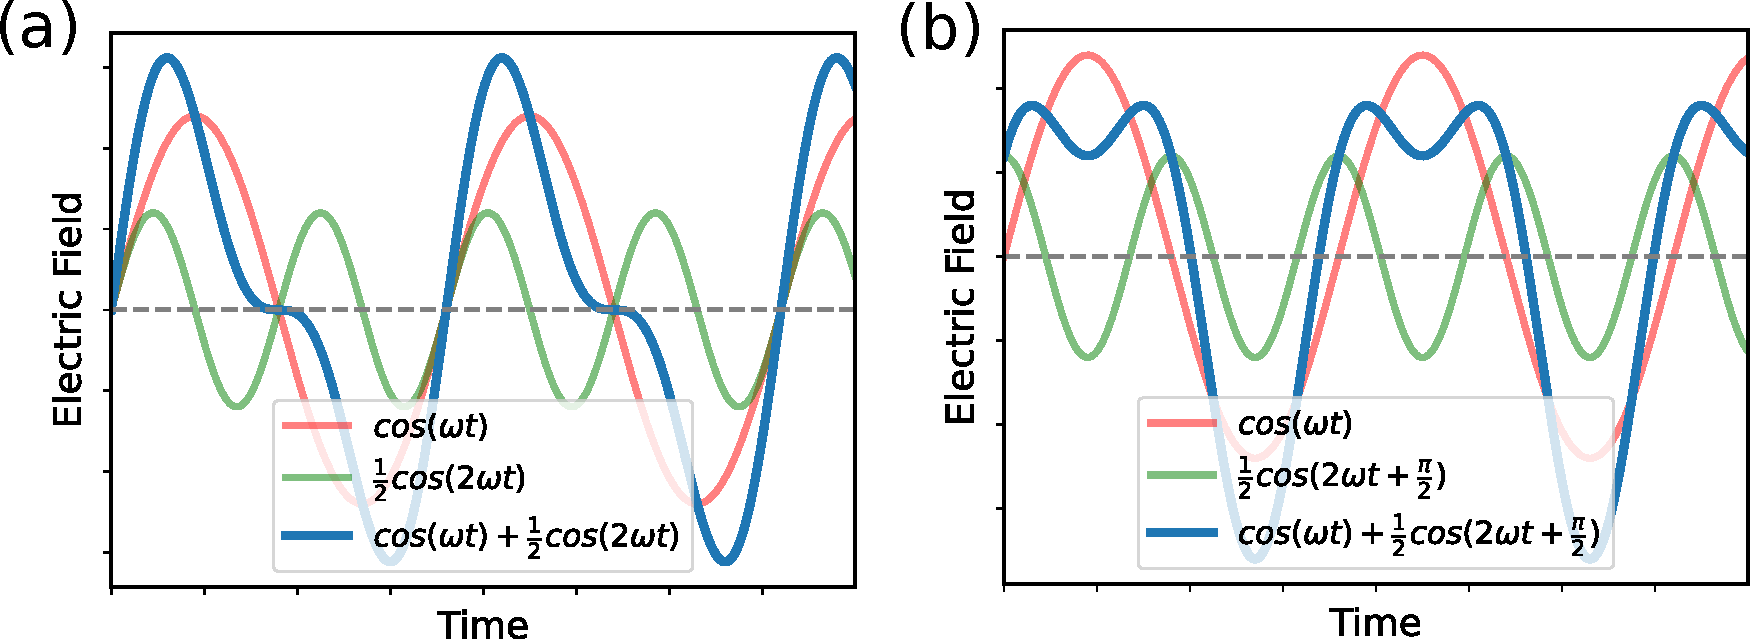
\includegraphics[width=1.0\linewidth]{pic/electric.pdf}
\caption{\label{fig:electricfield} 
The time profiles of the electric field given by Eq.~(\ref{eq:ele-pot-w-2w}) are shown for (a) $\phi=0$ and (b) $\phi=\pi/2$. The corresponding vector potential is shown in (c) $\phi=0$ and (d) $\phi=\pi/2$.}
\end{figure}


To comprehensively determine the persistent dc-current following laser irradiation, we conduct an in-depth analysis utilizing the photo-excited conduction population $n_{c\mathbf{k}}$ computed from Eq.~(\ref{eq:population_tdse}): 
\begin{align}
n_{c\vecb{k}} = \left | \langle \phi_{c \vecb{k}} | \psi_{\vecb{k}}(t_F) \right |^2,
\end{align}
where $t_F$ is a time after the laser field ends ($t_F>\tau/2$).
Employing a weak enough laser field in the perturbation region with a strength of $E_0=2.57$~MV/cm and fixing the relative phase at $\phi=0$, the resulting conduction population is illustrated in Fig.~\ref{fig:population}~(a). For comparative purposes, Fig.~\ref{fig:population}~(b) presents the conduction population $n_{c\mathbf{k}}$ computed under the same field strength ($E_0=2.57$~MV/cm) but with a distinct relative phase ($\phi=0$). In both instances, the conduction populations exhibit notable excitations centered around the $K$- and $K'$-points. This observation implies that the photo-absorption process is primarily governed by a one-photon absorption at the photon energy of $2\hbar \omega$ and a two-photon absorption at the photon energy of $\hbar \omega$. The consistency in the excitation patterns further underscores the dominance of these absorption mechanisms in the system under the specified laser conditions.


While the population distributions in Fig.\ref{fig:population}(a) and (b) may initially appear similar, a closer examination reveals distinctions. In the case of the time-reversal symmetry-broken field ($\phi=0$) illustrated in Fig.\ref{fig:population}(a), the population distribution must show an imbalance between time-reversal pairs (e.g., $\mathbf{k}$ and $-\mathbf{k}$, or $K$ and $K'$). On the contrary, in the case of the time-reversal field ($\phi=\pi/2$) showed in Fig.\ref{fig:population}(b), the population distribution $n_{c\mathbf{k}}$ is anticipated to lack such a population imbalance. This discrepancy arises from the absence of a persistent current under these conditions. This analysis deepens our understanding of the complicated relationship between population distributions and the underlying time-reversal symmetry characteristics, providing crucial insights into the dynamic behavior of the system.

\begin{figure}[htbp]
\centering
 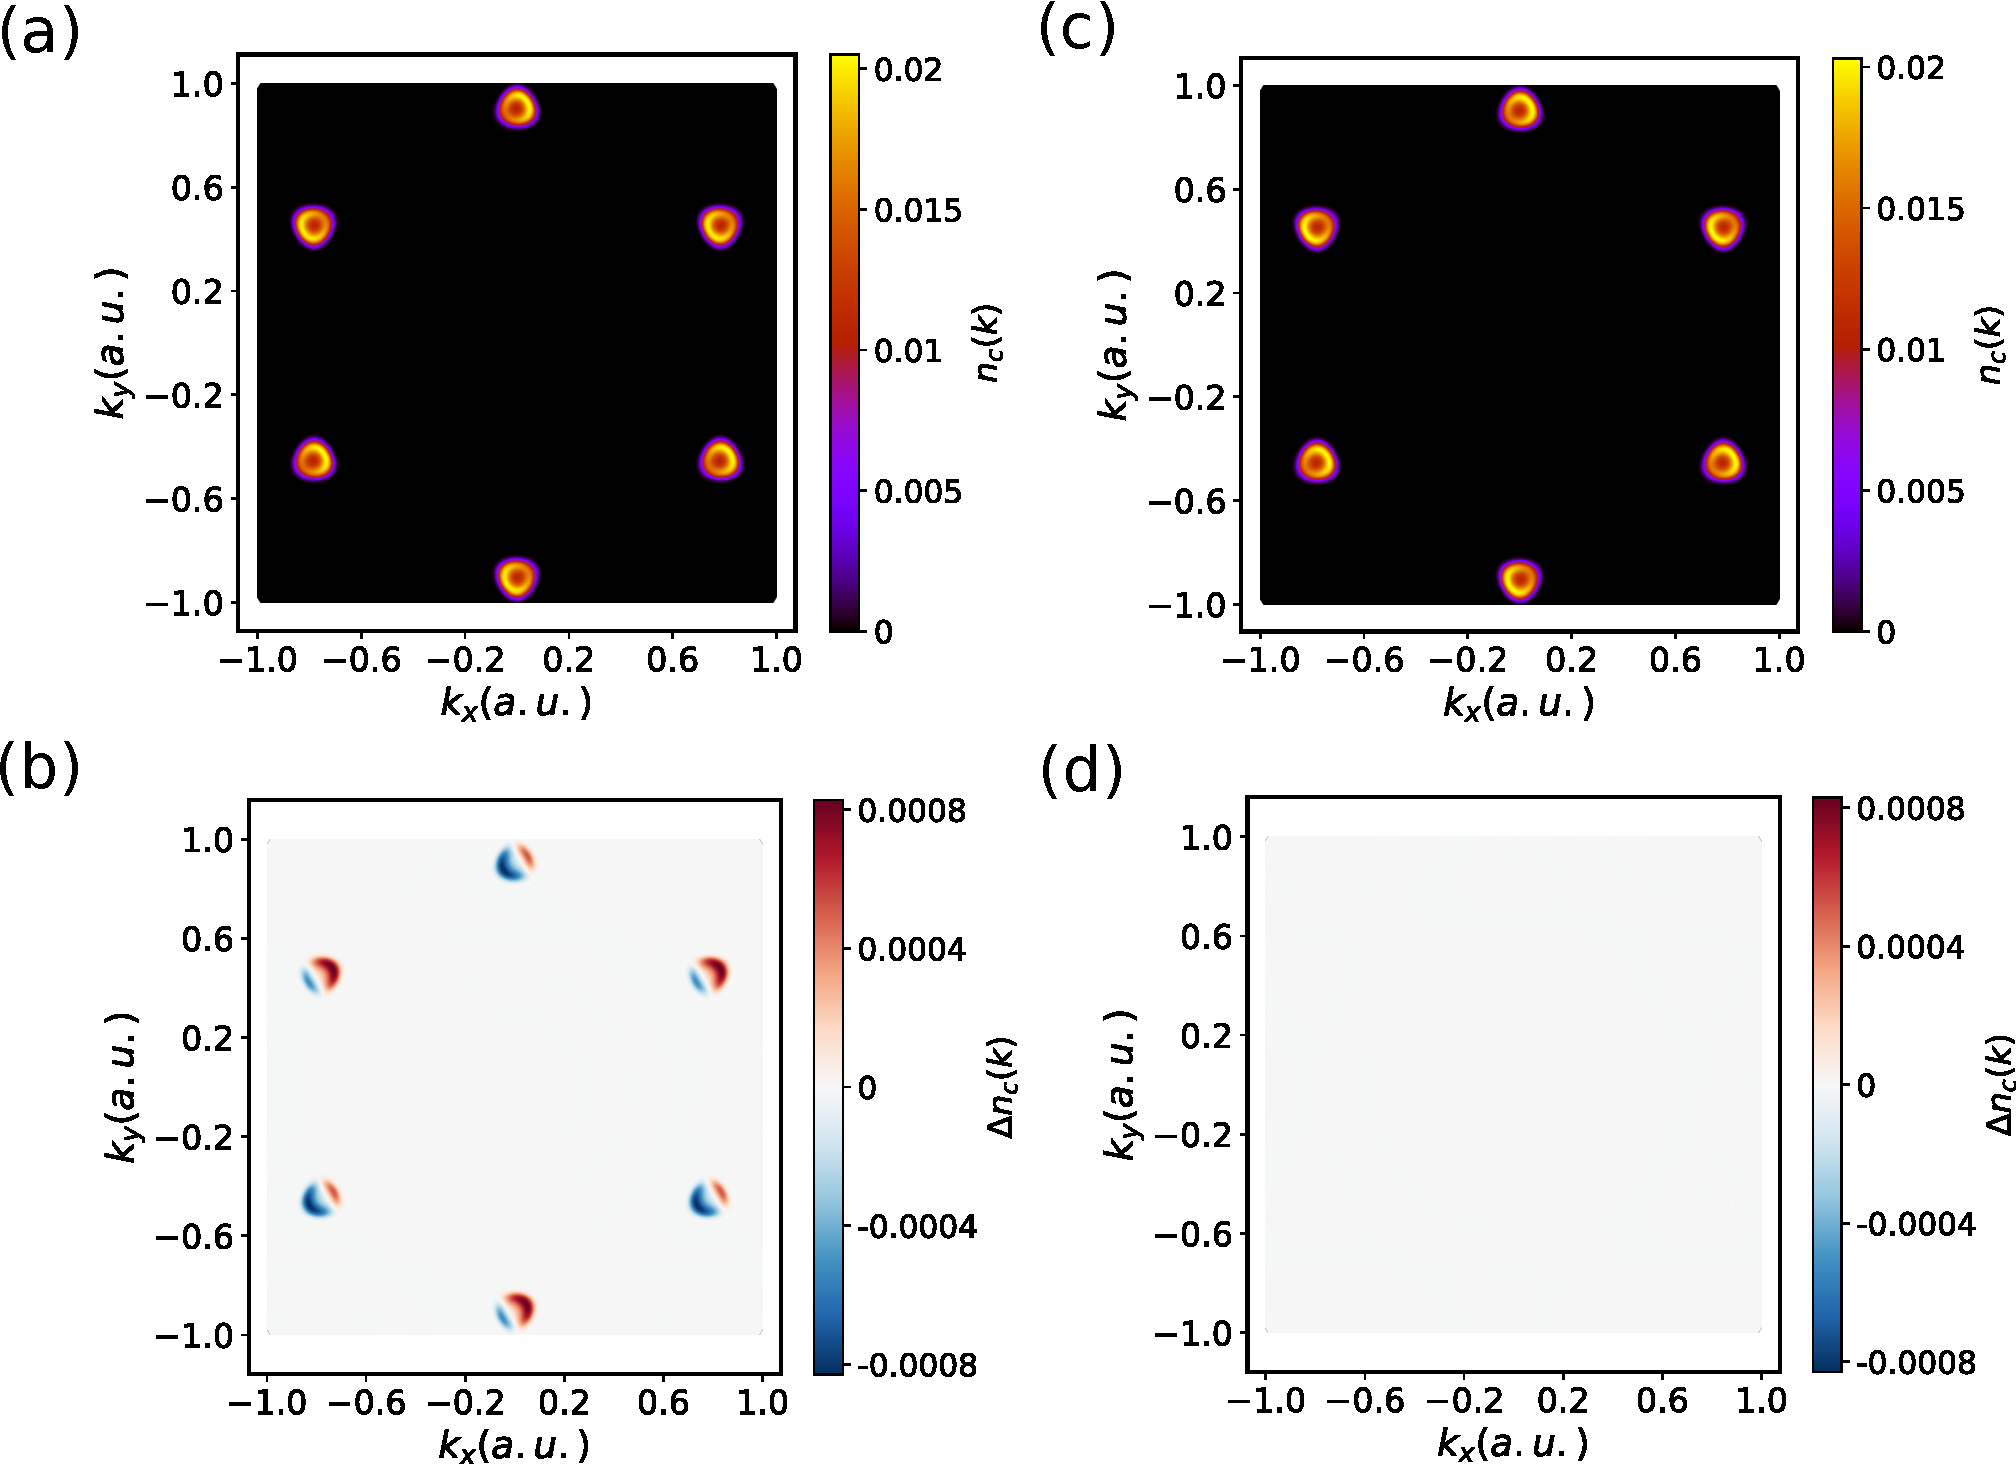
\includegraphics[width=1.0\linewidth]{pic/population.pdf}
\caption{\label{fig:population} 
(a, b) The conduction population distribution $n_c(\mathbf k)$ computed with (a) $\phi=0$ and (b) $\phi=\pi/2$. (c, d) The population imbalance distribution $\Delta n_c(\mathbf k)$ computed with (c) $\phi=0$ and (d) $\phi=\pi/2$.}
\end{figure}


To delineate the population imbalance across the Brillouin zone, we introduce the population imbalance distribution $\Delta n_{c\mathbf{k}}$, defined as the disparity in population between the time-reversal pair $k$-points, expressed as:
\begin{equation}
 \Delta n_{c\mathbf{k}}=n_{c\mathbf{k}}-n_{c, -\mathbf{k}}  
\label{pop_imbalance }
\end{equation}
Given the constraint $0 \le n_{c\mathbf{k}} \le 1$, the population imbalance distribution is bounded by $-1 \le \Delta n_{c\mathbf{k}} \le 1$. In situations where external fields maintain time-reversal symmetry, the populations at $\mathbf{k}$ and $-\mathbf{k}$ are equivalent, resulting in a population imbalance distribution of zero. Conversely, in instances where time-reversal symmetry is broken, non-equivalent populations can be induced at $\mathbf{k}$ and $-\mathbf{k}$, giving rise to a finite population imbalance distribution $\Delta n_{c\mathbf{k}}$.
Figures~\ref{fig:population}(c) and (d) illustrate the population imbalance distribution, $\Delta n_{c\mathbf{k}}$, derived from the population distributions presented in Figs.\ref{fig:population}~(a) and (b), respectively. The figures clearly illustrate that when the external field disrupts time-reversal symmetry ($\phi=0$), a discernible finite population imbalance is induced. In contrast, when the field preserves time-reversal symmetry ($\phi=\pi/2$), the population imbalance diminishes entirely. This comprehensive analysis of the population imbalance distribution provides a detailed insight into the complicated interplay between external field characteristics and the resulting population asymmetry within the Brillouin zone.


The temporal evolution of the corresponding electric current, denoted as $\mathbf{J}_{total}(t)$, can be computed using Eq.(\ref{eq:current}). This equation represents a functional dependence on the vector potential $\mathbf{A}(t)$, as illustrateed in Fig.\ref{fig:initial_current}. The total current encompasses multiple components and noises, often overshadowing the relatively small value of the dc-component following the laser pulse. To examine and isolate the dc-current generated by the fields, we introduce the global phase $\theta$ into the fields as described by the Eq.(\ref{eq:vec-pot-w-2w}), as done in our prior study\cite{sato2023limitations}.
\begin{equation}
\mathbf{A}(t) = -\mathbf{e}_p \frac{E_0}{\omega} \left [
\cos \left (\omega t + \theta \right ) + \frac{1}{4}\cos
\left (2\omega t + 2\theta + \phi \right )
\right ] \times \cos^4 \left (\frac{\pi}{\tau}t \right )
\label{eq:vec-pot-w-2w}
\end{equation}

\begin{figure}[htbp]
\centering
 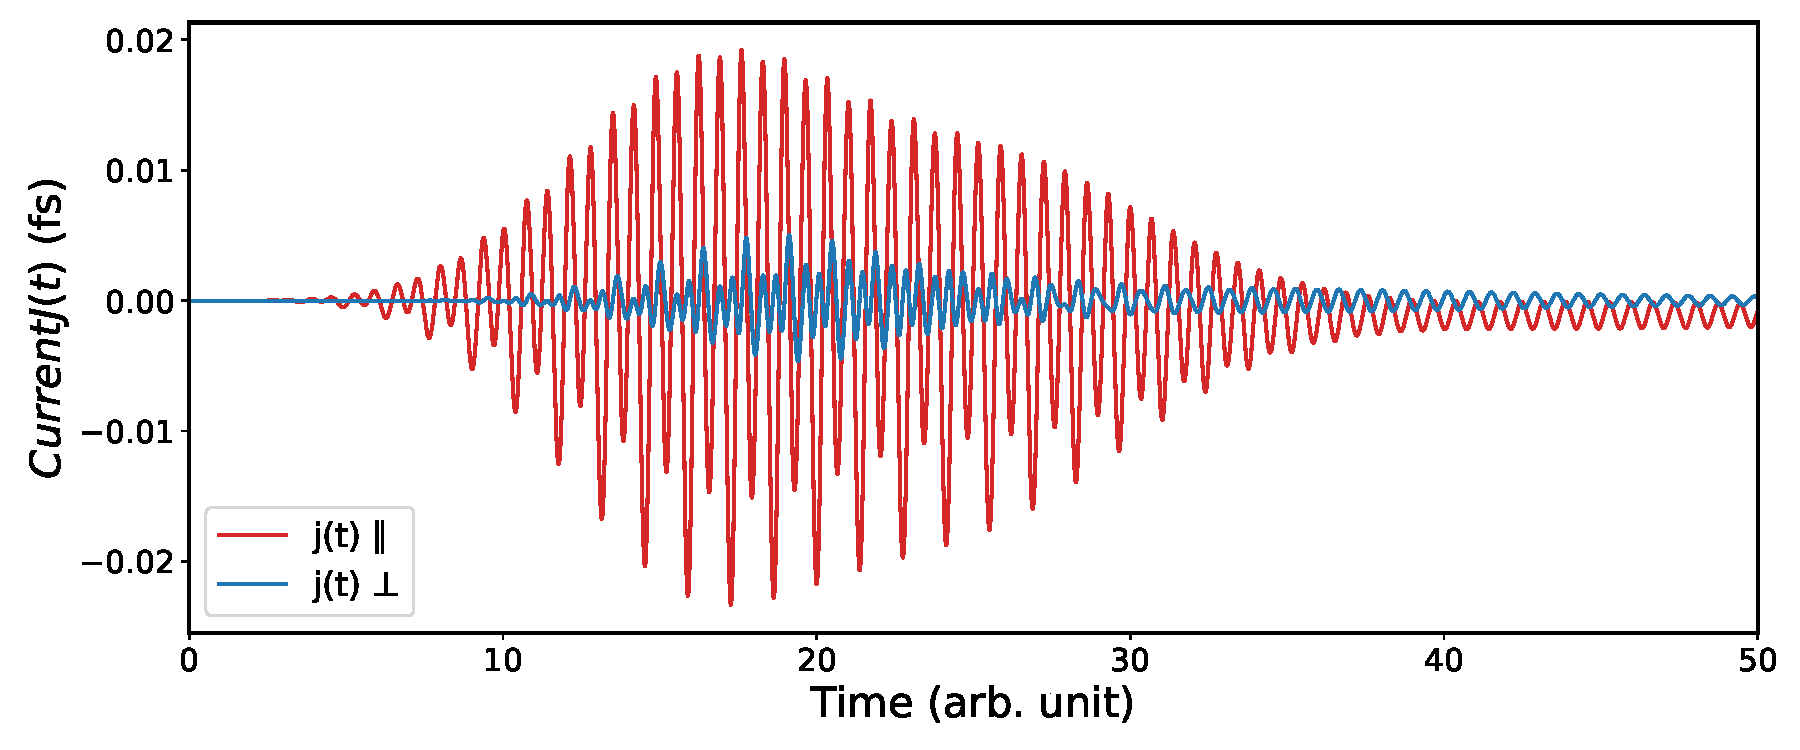
\includegraphics[width=1.0\linewidth]{pic/initial_current.pdf}
\caption{\label{fig:initial_current}} 
The time profiles of the current computed from Eq.~(\ref{eq:current}) induced by the electric field given by Eq.~(\ref{eq:ele-pot-w-2w}) as shown in Fig. ~\ref{fig:electricfield}(a) with relative phase $\phi=0$. 
\end{figure}
The current, expressed as a function of the global phase $\theta$ in accordance with the vector potential given by Eq.(\ref{eq:vec-pot-w-2w}), is explicitly denoted as $\mathbf{J}(t,\theta)$. By maintaining all laser parameters constant in Eq.(\ref{eq:vec-pot-w-2w}) except for the global phase $\theta$, we can isolate the direct current (dc)-like component of the induced current through the following integral:
\begin{equation}
\mathbf{J}_{\text{dc}}(t) = \frac{1}{2\pi} \int_0^{2\pi} d\theta , \mathbf{J}(t,\theta).
\label{eq:dc-current}
\end{equation}
In this formulation, the integral averages out the higher-frequency components, enabling the extraction of the clean dc-like slow-frequency component of the induced current.
\begin{figure}[htbp]
\centering
 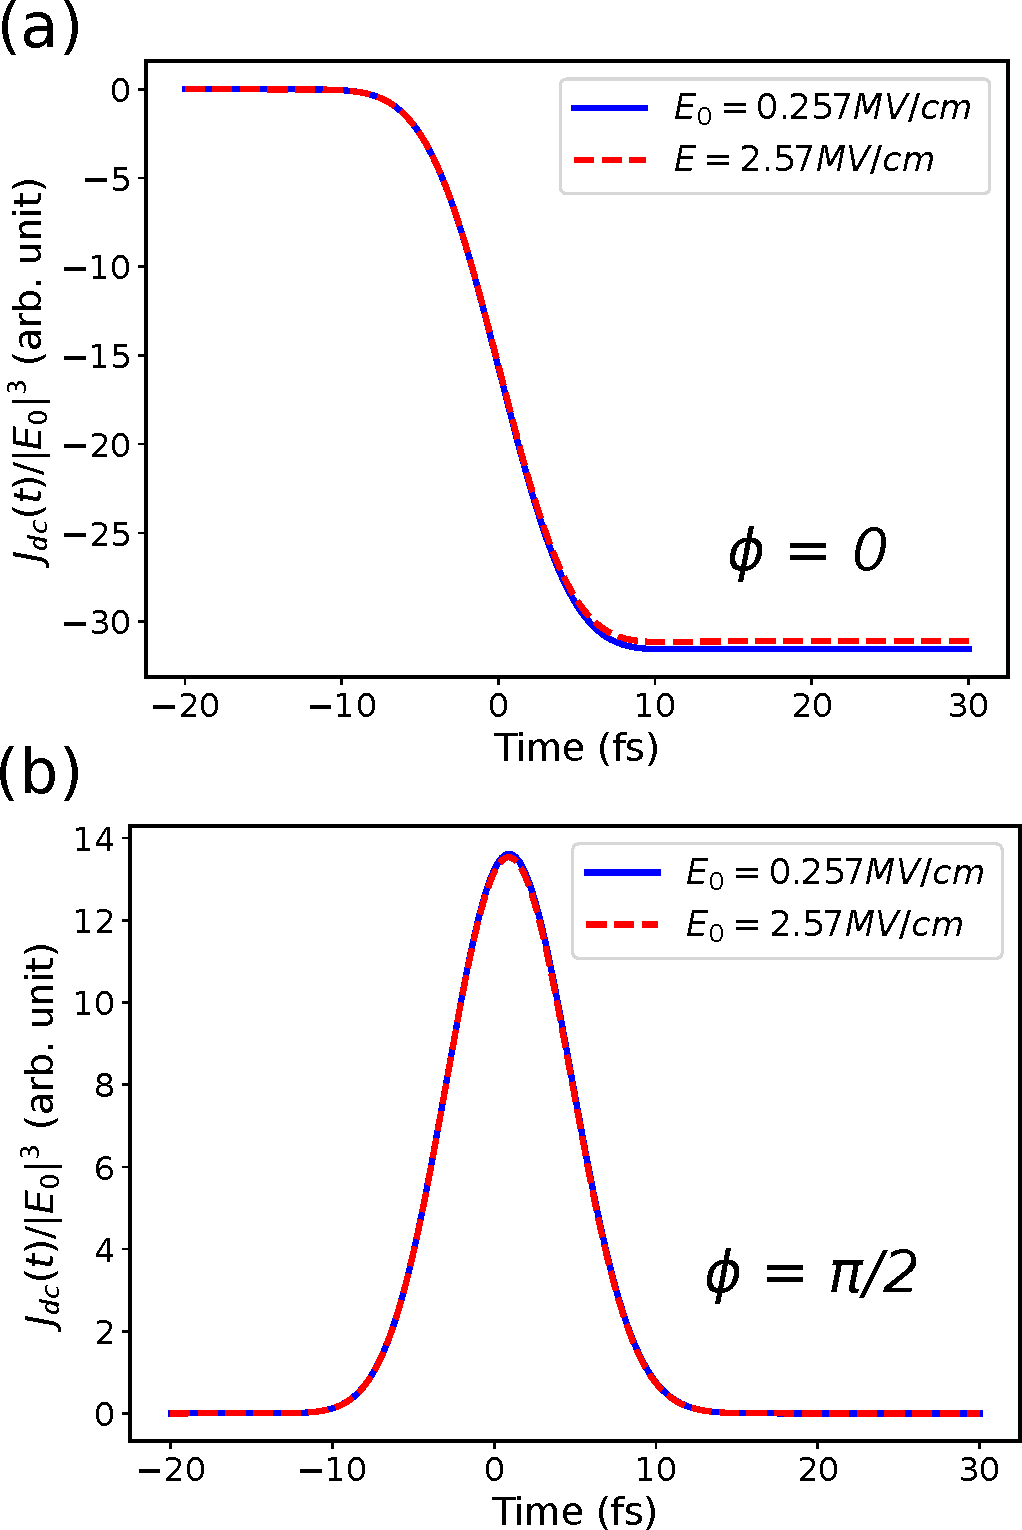
\includegraphics[width=0.8\linewidth]{pic/dc_current.pdf}
\caption{\label{fig:dc_current} 
The dc components of the currents $\mathbf{J}_{\text{dc}}(t)$ computed from Eq.~(\ref{eq:dc-current}) are shown as a function of time. The results using the relative phase of $\phi=0$ are shown in panel (a), while those using $\phi=\pi/2$ are shown in (b) }
\end{figure}

In Figure~\ref{fig:dc_current}(a), the calculated dc-current component of the scaled current, $\mathbf{J}_{\text{dc}}(t)/E_0^3$, is presented for a relative phase of $\phi=0$, including results for various field strengths, $E_0$. Remarkably, the residual dc-current persists beyond the conclusion of the laser fields ($t>\tau/2$). Notably, the scaled quantity, $\mathbf{J}{\text{dc}}(t)/E_0^3$, maintains identical behavior across different field strengths. This consistency suggests that the dc component of the induced current can be interpreted as a third-order nonlinear optical effect. This interpretation aligns with the inherent nature of the 1+2 \gls{QuIC} process, which involves interference between one- and two-photon absorption processes, classifying it as a third-order nonlinear optical phenomenon. The presented results shed light on the robust and field-independent nature of the observed third-order nonlinear optical effects in the system.

In Figure~\ref{fig:dc_current}(b), the dc-current component of the scaled current, $\mathbf{J}_{\text{dc}}(t)/E_0^3$, is illustrateed with a relative phase of $\phi=\pi/2$. In stark contrast to the results with $\phi=0$ shown in Fig.\ref{fig:dc_current}(a), the currents in Fig.\ref{fig:dc_current}~(b) do not show a persistent dc component after the conclusion of the laser irradiation. This outcome signifies that the applied field with a relative phase of $\phi=\pi/2$ does not disrupt time-reversal symmetry, and consequently, no population imbalance is induced, resulting in the absence of a sustained current. It is noteworthy that, even in the case of $\phi=\pi/2$, the dc-component of the current is induced solely during the laser irradiation, highlighting yet another instance of a third-order nonlinear optical process. This observation provides further insight into the nuanced interplay between field characteristics and the resulting dynamical responses in the system.


By manipulating the relative phase $\phi$, one gains control over the extent of time-reversal symmetry breaking, thereby influencing the resulting population imbalance and dc- current injection~\cite{PhysRevLett.74.3596}. For subsequent analysis, we systematically explore the persistent dc current by varying the relative phase $\phi$. Figure~\ref{fig: imbalance} illustrates the dependence of the dc-current on the relative phase $\phi$ after laser irradiation, computed using a field with a strength of $E_0=2.57~$MV/cm. The amplitude of the induced dc current reaches its maximum when $\phi=0$ and $\phi=\pi$, with opposite signs for these two phases. Moreover, the induced dc current exhibits continuous variation as the phase $\phi$ is manipulated, attaining zero when $\phi=\pi/2$ and $\phi=3\pi/2$, corresponding to the points where the applied fields restore time-reversal symmetry. This straightforward phase dependence aligns with findings from prior works\cite{PhysRevLett.74.3596,PhysRevLett.78.306}, providing further validation of the controllable nature of the induced dc current through manipulation of the relative phase.

\begin{figure}[htbp]
\centering
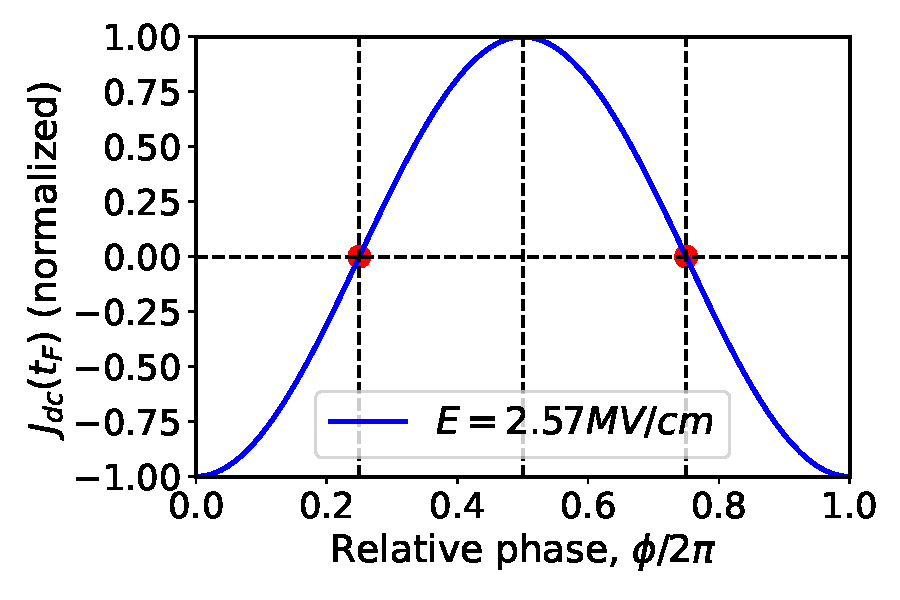
\includegraphics[width=0.8\linewidth]{pic/relativephase.pdf}
\caption{\label{fig: imbalance} 
The persistent current $J_{\text{dc}}(t_f)$ as a function of the relative phase, $\phi$. The results are computed by setting $E_0$ to $2.57$~MV/cm and $\hbar \omega$ to 3~eV.}
\end{figure}


\gls{QuIC} processes often exhibit resonance conditions at specific photon energies. By systematically investigating the photon-energy dependence, we can identify resonant regions where the interference effects are significantly enhanced.  Investigating these dependencies helps identify the primary mechanisms. To investigate this phenomenon within our theoretical framework, we systematically evaluate the direct current (dc) after laser irradiation by varying the fundamental frequency $\omega$ in Eq.(\ref{eq:vec-pot-w-2w}). Figure\ref{fig:fig4}~(a) illustrates the resulting dc current following laser irradiation with a field strength of $E_0=1.03$~MV/m. 

According to the expected behavior of the $1+2$~\gls{QuIC} process, the dc-current decreases when the fundamental photon energy falls below half of the band gap, i.e., $\hbar \omega \le E_g/2 = 2.95$~eV,  since the fundamental photon energy $\hbar \omega$ must adhere to the condition $\hbar \omega \ge E_g/2$, where $E_g$ signifies the band gap. 
In instances where the fundamental photon energy $\hbar \omega$ falls below the gap, both the $1+2$~QuIC process and the resultant dc-current vanish. This exploration not only clarify the crucial role of photon energy in the indication of the $1+2$~\gls{QuIC} process but also underscores the significance of satisfying specific conditions for its occurrence and subsequent dc-current induction.
This behavior aligns with the expected characteristics of the $1+2$~\gls{QuIC} process and provides valuable insights into the influence of the fundamental frequency on the induced dc-current in our theoretical framework.
\begin{figure}[htbp]
\centering
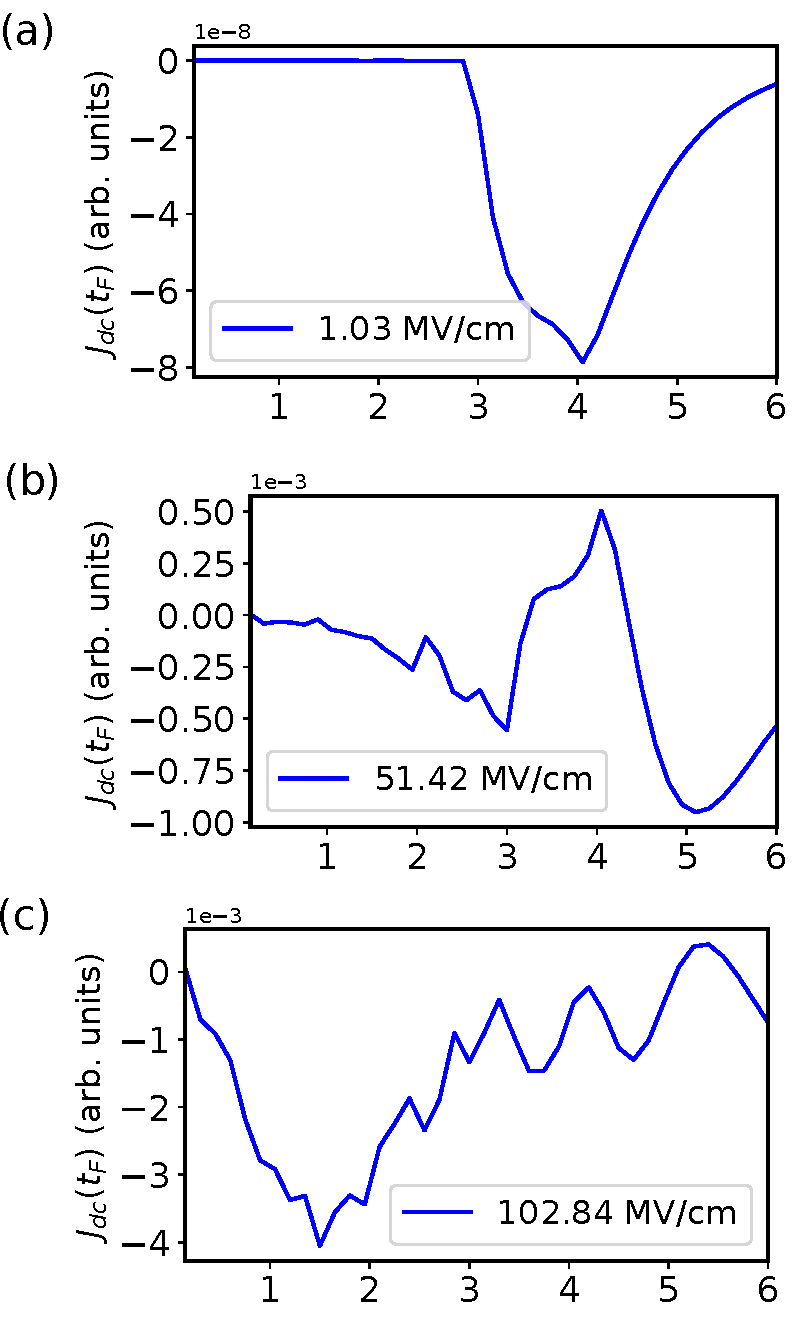
\includegraphics[width=0.8\linewidth]{pic/frequency.pdf}
\caption{\label{fig:fig4} 
The current after the laser irradiation is shown as a function of the fundamental photon energy $\hbar \omega$. The results computed different field strengths: (a) $E_0=1.03$~MV/cm, (b) $51.43$~MV/cm, and (c) $E_0=102.84$~MV/cm.}
\end{figure}

 The investigation helps understand the complicated relationship between photon energy, field strength, and the nonlinear processes. It is essencial to investigate the photon energy dependence of the dc-current after laser irradiation while varying the field strength, $E_0$, to unravel the intricacies of this highly nonlinear optical phenomenon. 
 Figures~\ref{fig:fig4}~(b) and (c) throughly illustrate the photon-energy dependence of the persistent current following laser irradiation, calculated for two distinct field strengths: (b) $E_0=51.42$~MV/cm and (c) $E_0=102.84$~MV/cm. In contrast to the weak field regime dominated by the $1+2$~\gls{QuIC}, the direct current (dc) can be induced even under deeply off-resonant conditions, where the photon energy is smaller than half of the band gap ($\hbar \omega \le E_g/2$), as evident in Figure\ref{fig:fig4}(b). This convincing observation suggests that potent laser fields introduce additional pathways for electron excitation that extend beyond two-photon absorption. These additional processes, involving multiple photons, contribute to the creation of a population imbalance and a dc-current, even in the deeply off-resonant regime. The interaction between laser field strength and photon energy unveiled in these results provides invaluable insights into the complex dynamics governing persistent currents in strong-field regimes.

 Illustrated in Figure~\ref{fig:fig4}~(c), a noteworthy observation emerges the magnitude of the direct current (dc) after laser irradiation in the deeply off-resonant regime ($\hbar \omega \le E_g/2$) surpasses that in the $1+2$~\gls{QuIC} regime ($\hbar \omega \ge E_g/2$) as the applied field strength reaches exceptionally large values. This interesting behavior finds its explanation in the ponderomotive energy, denoted as:
 \begin{align}
 U_p=\frac{e^2E^2_0}{4m\pi \omega_0^2}    
 \end{align}
 The associated light-induced intraband transitions, both of which are more substantial for lower frequency driving\cite{PhysRevB.98.035202}. Consequently, the ensuing nonlinear effects and the injection of dc current become more pronounced in the deeply off-resonant regime compared to the resonant condition. 
Our initial investigation focused on analyzing the electric current induced by these two-color laser fields within the weak field regime. We confirmed that the dc-component of the induced current persists even after laser irradiation when the fundamental photon energy $\hbar \omega$ exceeds the optical gap, $E_g/2$. This ballistic current phenomenon originates from a population imbalance in the Brillouin zone, arising from quantum interference between two distinct excitation paths: one involving one-photon absorption at the photon energy of $2\hbar \omega$, and the other involving a two-photon absorption path at the photon energy of $\hbar \omega$~\cite{PhysRevLett.74.3596,PhysRevLett.76.1703,PhysRevLett.78.306}.


 This discovery sets the stage for a more in-depth exploration in the subsequent section, where we will study into the involvements of efficiently inducing dc-current through highly nonlinear optical processes in the deeply off-resonant regime.


%%%%%%%%%%%%%%%%%%%%%%%%%%%%%%%%%%%%%%%%%%%%%%%%%%%%%%%%%%%%%%%%%%%%%%%%%%%%%%%%%%%
\section{Deeply Off-resonant Highly-nonlinear Regime \label{sec:nonperturbative}}
%%%%%%%%%%%%%%%%%%%%%%%%%%%%%%%%%%%%%%%%%%%%%%%%%%%%%%%%%%%%%%%%%%%%%%%%%%%%%%%%%%%

Despite the significant interest in the nonlinear photovoltaic effect, there has been limited exploration of efficient current injection in the deeply off-resonant regime with multi-cycle light pulses, particularly using linearly polarized light. Subsequently, the scope of \gls{QuIC} can be extended to involve general integer combinations, denoted as $M+N$~\gls{QuIC}~\cite{PhysRevB.100.075202,PhysRevLett.123.067402}. In this extended scheme, two-color laser fields operating at frequencies $\omega$ and $\omega'$ induce $M$- and $N$-photon absorption processes, respectively.
To investigate the mechanism of dc-current injection in the deeply off-resonant regime, as demonstrated in the previous section, we fix the fundamental photon energy $\hbar \omega$ in Eq.~(\ref{eq:vec-pot-w-2w}) at $1$~eV. Notably, this value is much smaller than half of the band gap, $E_g/2=2.95$~eV, for this section.

\begin{figure}[htbp]
\centering
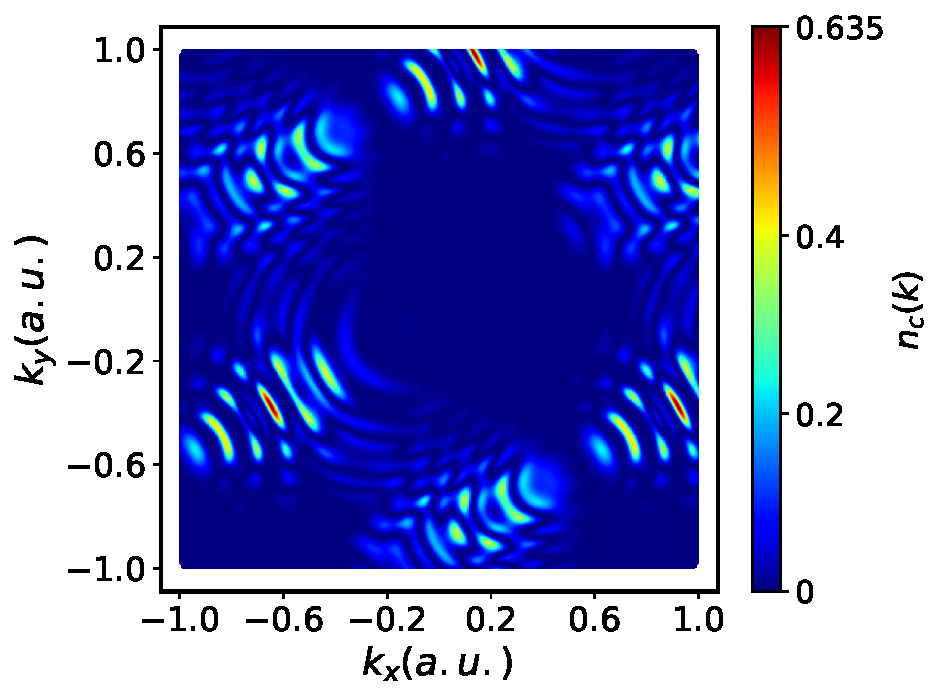
\includegraphics[width=0.8\linewidth]{pic/nex_pop_E0_1e10.pdf}
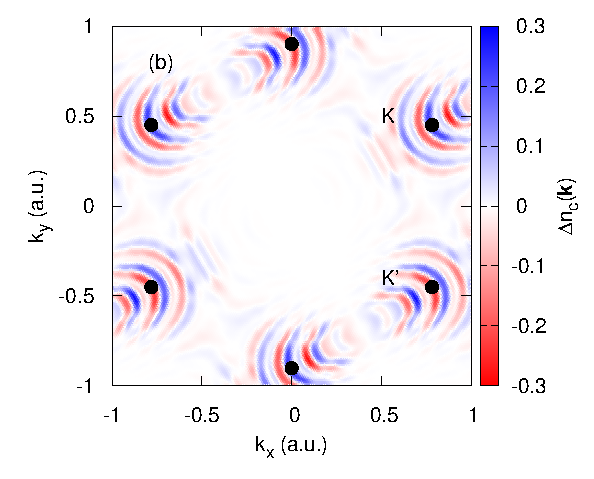
\includegraphics[width=0.8\linewidth]{pic/dnex_pop_E0_1e10.pdf}
\caption{\label{fig:nex_pop_E0_1e10} 
(a) The conduction population distribution $n_{c}(\mathbf k)$ after the irradiation of the laser field, and (b) the population imbalance distribution $\Delta n_c (\mathbf k)$ are shown. The results are computed by setting $E_0$ to $10^{10}$~V/m.
}
\end{figure}

Similarly, we start with evaluating the population imbalance induced by a strong field in the
deeply off-resonant regime, we calculate the population distribution $n_{c\vec{k}}$ after
irradiating the laser field with a strength of $100$~MV/cm. A distinct pattern emerges in the excited carrier population distribution around the $K$ and $K'$ points. This pattern can be understood through the multi-photon absorption resonances of the light-induced Floquet states\cite{galler2023mapping}. In Fig.\ref{fig:nex_pop_E0_1e10}(a), we present the computed population distribution in the conduction band. As anticipated from the preceding discussion, the photo-carrier distribution reveals a significant population imbalance between $\mathbf{k}$ and $-\mathbf{k}$ points. To enhance clarity in visualizing the population imbalance, we compute the population imbalance distribution $\Delta n_{c\mathbf{k}}=n_{c\mathbf{k}}-n_{c, -\mathbf{k}}$. Figure~\ref{fig:nex_pop_E0_1e10}(b) displays the resulting population imbalance distribution $\Delta n_{c\mathbf{k}}$. Since $\Delta n_{c\mathbf{k}}$ is constrained by $-1\le \Delta n_{c\mathbf{k}} \le 1$, the population imbalance between $\mathbf{k}$ and $-\mathbf{k}$ is maximized when $|\Delta n_{c\mathbf{k}}|=1$. As observed in Fig.\ref{fig:nex_pop_E0_1e10}~(b), the population imbalance distribution takes significantly large values, comparable to the maximum values ($\pm 1$), across a wide range of the Brillouin zone.
\begin{figure}[htbp]
\centering
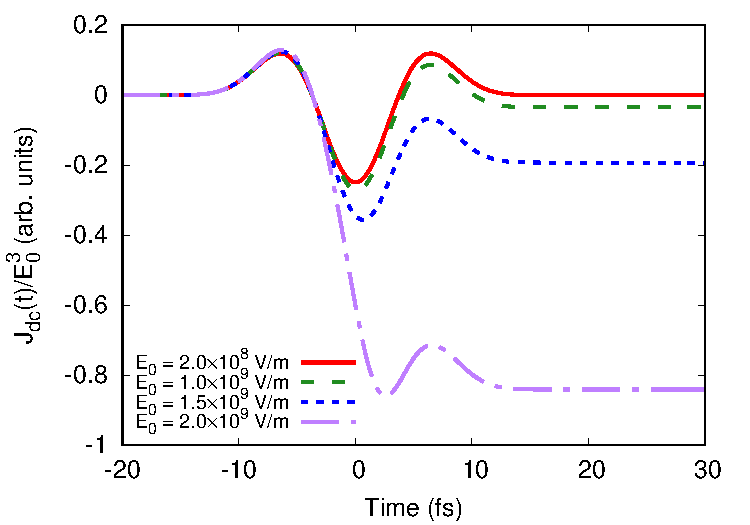
\includegraphics[width=0.8\linewidth]{pic/current_off_resonant.pdf}
\caption{\label{fig:current_off_resonant} 
The dc components of the currents, $\mathbf J_{dc}(t)$, are shown as a function of time. The results are computed with the deeply off-resonant condition, $\hbar\omega = 1.0$~eV.}
\end{figure}

We calculate the population imbalance ratio $r_{im}$ defined as the maximum absolute value of the
population imbalance distribution $\Delta n_{c\mathbf{k}}$ across the Brillouin zone for further
qualification. Mathematically, it is expressed as:
\begin{equation}
r_{im} = \frac{\int_{BZ}d\mathbf k \left |\Delta n_{c\mathbf{k}} \right |}{\int_{BZ}d\mathbf k \left (n_{c\mathbf{k}} + n_{c,-\mathbf{k}}\right )}
= \frac{\int_{BZ}d\mathbf k \left |\Delta n_{c\mathbf{k}} \right |}{2\int_{BZ}d\mathbf k n_{c\mathbf{k}}}.
\end{equation}
The computed imbalance ratio, $r_{im}$, from Figs.\ref{fig:nex_pop_E0_1e10}(a) and (b) is about
0.307. Hence, more than 30\% of the excited electrons contribute to the population imbalance.
This implies the potential for realizing a significant population imbalance through the use of linearly polarized light alone.

In an earlier study~\cite{Jimenez-Galan2020}, significant control over valley population was proposed using bi-circular fields with counter-rotating $\omega$ and $2\omega$ two-color laser fields. In contrast, in this work, we demonstrate that significant valley population can be induced without relying on circular or elliptically polarized light; rather, bi-color linearly polarized light alone can break the time-reversal symmetry and cause such population control.


We commence our analysis of population imbalance by examining the light-induced current in the time domain within the deeply off-resonant regime. In Figure~\ref{fig:current_off_resonant}, we present the dc component of the current, $\mathbf{J}_{\text{dc}}(t)/E_0^3$, computed with varying field strengths, $E_0$. For this analysis, the relative phase $\phi$ is set to 0. Evidently, a third-order nonlinear response dominates the induced current in the case of weak field strength. Given that the photon energy of the second harmonic is smaller than the band-gap ($2\hbar \omega < E_g$) and the \gls{QuIC} process is forbidden, the third-order current returns to zero after the laser irradiation.

However, as the field strength becomes sufficiently strong, the dc-component remains finite even after laser irradiation, as illustrateed in Fig.~\ref{fig:current_off_resonant}. This observation suggests that a higher-order nonlinear process contributes to the ballistic dc-current injection beyond the third-order nonlinear effect.

\begin{figure}[htbp]
\centering
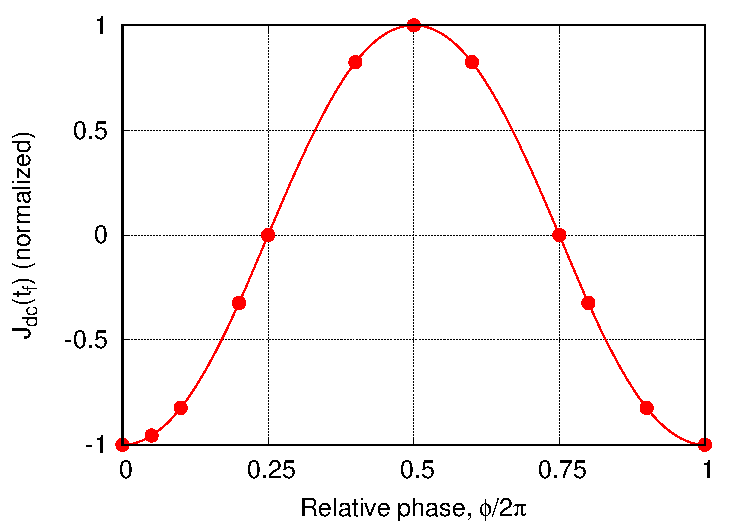
\includegraphics[width=0.8\linewidth]{pic/jdc_vs_phi_off_resonance.pdf}
\caption{\label{fig:jdc_vs_phi_off_resonance} 
The persistent current, $J_{dc}(t_f)$, is shown as a function of the relative phase $\phi$. The results are computed with the deeply off-resonant condition, $\hbar\omega = 1.0$~eV.
}
\end{figure}

Next, we explore the dependence of the ballistic current induced by deeply off-resonant light on
the relative phase, $\phi$. Figure~\ref{fig:jdc_vs_phi_off_resonance} illustrates the computed
current as a function of the relative phase, $\phi$, with calculations conducted at a field
strength of $E_0=1 \times 10^{4}$ MV/m. In accordance with the QuIC case shown in Fig.\ref{fig:
imbalance}, the persistent current is maximized when the relative phase is $\phi=0$ or $\phi=\pi$,
and it vanishes when the applied field exhibits time-reversal symmetry ($\phi=\pi/2$ or
$\phi=3\pi/2$). Therefore, even in the deeply off-resonant regime, the direction and magnitude of
the persistent current can be controlled by manipulating the relative phase $\phi$ between the
two-color fields at frequencies $\omega$ and $2\omega$.\\

\begin{figure}[htbp]
\centering
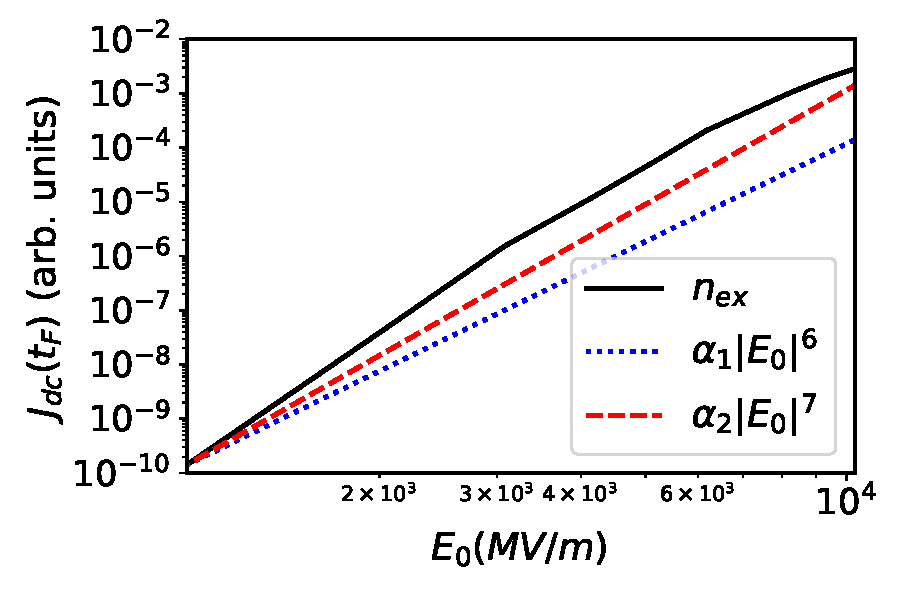
\includegraphics[width=0.80\linewidth]{pic/dc_current_vs_E0.pdf}
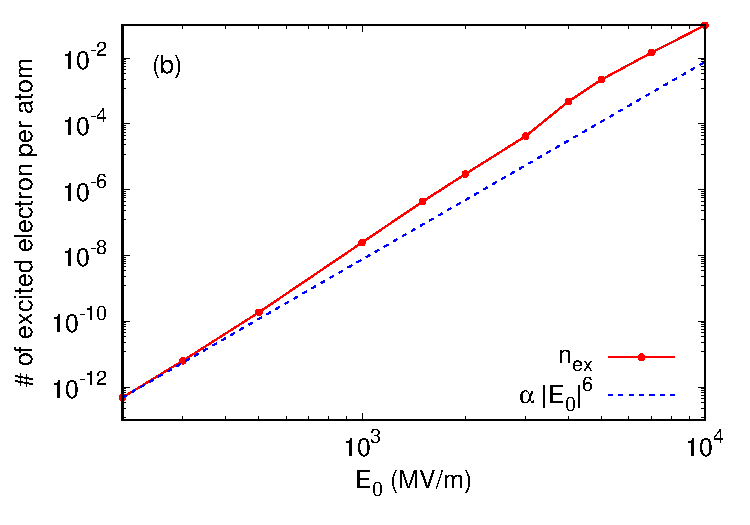
\includegraphics[width=0.80\linewidth]{pic/nex_vs_E0.pdf}
\caption{\label{fig:dc_current_vs_E0} 
(a) The persistent current, $|J_{dc}(t_f)|$, is shown as a function of the field strength, $E_0$. (b) The number of conduction population after the laser irradiation is shown as a function of the field strength $E_0$.
}
\end{figure}
To gain a more detailed understanding of the complicated mechanism behind dc current injection in the deeply off-resonant regime, we study into an analysis of how the injected current scales with the applied field strength $E_0$. As illustrateed in Figure~\ref{fig:dc_current_vs_E0}, the current amplitude after laser irradiation is plotted against the varying field strength. Notably, a reference line representing $|E_0|^7$ is included for comparison.

The compelling observation from the figure is that the induced current exhibits a clear proportionality to $|E_0|^7$ in the weak field regime. This insightful finding suggests that the seventh-order nonlinear process takes precedence in governing the dynamics of dc current injection under these conditions. This nuanced understanding provides a comprehensive insight into the complicated nonlinear optical processes that contribute to the observed dc current phenomena in the deeply off-resonant regime.

The observed scaling law of the induced dc current with the applied field strength might initially
seem inconsistent with the expected behavior of a straightforward $M+N$ \gls{QuIC} process. In the
conventional $M+N$ \gls{QuIC} situation, the $M$-photon absorption process is initiated by light with frequency $\omega$, and the $N$-photon absorption process is generated by light with frequency $2\omega$, resulting in an overall $(M+N)$-th order nonlinear process. For instance, if we consider a six-photon process for multi-photon absorption with light of frequency $\omega$ and a three-photon process for light of frequency $2\omega$, the anticipated simple $M+N$ QuIC process corresponds to the ninth-order nonlinear process ($M+N=6+3=9$).

However, our experimental observations reveal a scaling that indicates seventh-order nonlinearity instead. This apparent discrepancy in the observed and expected nonlinearities of the injected dc current can be rationalized by the presence of an additional excitation channel involving a four-photon absorption process. In this situation, two photons at frequency $\omega$ and the other two photons at frequency $2\omega$ combine to excite electrons. This additional four-photon excitation channel interferes with the three-photon absorption process at the photon energy of $2\hbar \omega$, resulting in seventh-order ($7=3+4$) nonlinear current injection.

To study deeper into the nonlinearity of the light-induced electron dynamics, we performed computations to determine the number of photo-excited carriers after laser irradiation using the expression:
\begin{align}
N_{ex} = \frac{2}{A_{\mathrm{BZ}}}\int_{\mathrm{BZ}} d\mathbf{k} n_{c,\mathbf{k}}, 
\end{align}
where $A_{\mathrm{BZ}}=\int_{\mathrm{BZ}} d\mathbf{k}$ represents the area of the Brillouin zone.

Figure~\ref{fig:dc_current_vs_E0}~(b) presents the number of excited electrons as a function of the field strength, $E_0$, alongside a reference line proportional to $|E_0|^6$. In the weak field regime, the number of excited electrons exhibits proportionality to $|E_0|^6$, highlighting the dominance of the three-photon absorption process in the excitation mechanism. However, as the field strength increases, the deviation from the three-photon absorption line suggests the initiation of a nonperturbative mechanism in the excitation process.

In contrast to the $|E_0|^6$-dependence of the number of photo-excited carriers in the weak field regime, the injected current and the corresponding population imbalance follow a $|E_0|^7$ scaling, as illustrateed in Figure~\ref{fig:dc_current_vs_E0}~(a). The difference in nonlinearities between the absolute photo-carrier population and the population imbalance implies that the population imbalance is negligible concerning the absolute photo-carrier population in the weak field regime. However, in a strong field regime, the relative significance of the population imbalance becomes substantial as it grows more rapidly than the absolute photo-carrier population. Therefore, the distinction in nonlinearities between the total photocarrier population and the population imbalance indicates the potential for large-amplitude valley carrier population control.

Expanding our analysis to the deeply off-resonant regime, where $\hbar \omega \ll E_g/2$, we observed an absence of population imbalance under weak applied field strength. However, as the field strength increased, a population imbalance in the Brillouin zone is formed, leading to the injection of the persistent dc-current after the laser irradiation. Scaling analysis of the ballistic current injection with respect to the applied field strength $E_0$ revealed that the population imbalance and the ballistic current result from an interference between three-photon absorption process with three photons of energy $2\hbar \omega$ and a four-photon absorption process with two photons of energy $2\hbar \omega$ and two photons of energy $\hbar \omega$. Consequently, we demonstrated that a multi-photon absorption process, incorporating photons with different energies, plays a pivotal role in addition to the multi-photon absorption process involving single-color photons.


In previous works~\cite{Jimenez-Galan2020,Mrudul:21,PhysRevLett.127.126601}, the formation of substantial population imbalance and valley-population control has been discussed in monolayer systems such as monolayer $h$-BN and graphene, using bi-circular laser fields with frequencies $\omega$ and $2\omega$. Recently, valley-population control with bi-circular fields has been extended to multi-layer and bulk systems~\cite{tyulnev2023valleytronics} without relying on intrinsic inversion symmetry breaking and the Berry curvature at the valleys. In contrast to these works, our study demonstrates the induction of a large population imbalance and ballistic current injection without relying on the ellipticity of light. Instead, we rely on time-reversal symmetry breaking achieved through relative phase control between two-color linearly-polarized fields at frequencies $\omega$ and $2\omega$. Furthermore, similar to Ref.~\cite{tyulnev2023valleytronics}, the injection mechanism with bi-color linearly polarized light does not rely on intrinsic inversion symmetry breaking, indicating an efficient dc current injection and population control with the scheme using linearly-polarized light. The potential of population control and the photovoltaic effect with linearly polarized light, in addition to circularly/elliptically polarized light, unveils novel avenues for realizing ultrafast opto-electronics, marked by precise control of current and population dynamics on the femtosecond time scale.

